% This is "sig-alternate.tex" V2.1 April 2013
% This file should be compiled with V2.5 of "sig-alternate.cls" May 2012
%
% This example file demonstrates the use of the 'sig-alternate.cls'
% V2.5 LaTeX2e document class file. It is for those submitting
% articles to ACM Conference Proceedings WHO DO NOT WISH TO
% STRICTLY ADHERE TO THE SIGS (PUBS-BOARD-ENDORSED) STYLE.
% The 'sig-alternate.cls' file will produce a similar-looking,
% albeit, 'tighter' paper resulting in, invariably, fewer pages.
%
% ----------------------------------------------------------------------------------------------------------------
% This .tex file (and associated .cls V2.5) produces:
%       1) The Permission Statement
%       2) The Conference (location) Info information
%       3) The Copyright Line with ACM data
%       4) NO page numbers
%
% as against the acm_proc_article-sp.cls file which
% DOES NOT produce 1) thru' 3) above.
%
% Using 'sig-alternate.cls' you have control, however, from within
% the source .tex file, over both the CopyrightYear
% (defaulted to 200X) and the ACM Copyright Data
% (defaulted to X-XXXXX-XX-X/XX/XX).
% e.g.
% \CopyrightYear{2007} will cause 2007 to appear in the copyright line.
% \crdata{0-12345-67-8/90/12} will cause 0-12345-67-8/90/12 to appear in the copyright line.
%
% ---------------------------------------------------------------------------------------------------------------
% This .tex source is an example which *does* use
% the .bib file (from which the .bbl file % is produced).
% REMEMBER HOWEVER: After having produced the .bbl file,
% and prior to final submission, you *NEED* to 'insert'
% your .bbl file into your source .tex file so as to provide
% ONE 'self-contained' source file.
%
% ================= IF YOU HAVE QUESTIONS =======================
% Questions regarding the SIGS styles, SIGS policies and
% procedures, Conferences etc. should be sent to
% Adrienne Griscti (griscti@acm.org)
%
% Technical questions _only_ to
% Gerald Murray (murray@hq.acm.org)
% ===============================================================
%
% For tracking purposes - this is V2.0 - May 2012

% \documentclass{sig-alternate-05-2015}
% \usepackage{subcaption}
% \usepackage{subfig}
% \usepackage{multirow}
% %\usepackage{todo}
% \usepackage{soul}
% \usepackage{color}
% \usepackage[colorinlistoftodos]{todonotes}
% \begin{document}
% 
% % Copyright
% \CopyrightYear{2016} 
% \setcopyright{acmcopyright}
% \conferenceinfo{CIKM'16 ,}{October   24-November  28, 2016, Indianapolis, IN, USA}
% \isbn{978-1-4503-4073-1/16/10}\acmPrice{\$15.00}
% \doi{http://dx.doi.org/10.1145/2983323.2983675}
% %Authors, replace the red X's with your assigned DOI string.
% 
% \clubpenalty=10000 
% \widowpenalty = 10000
% %\setcopyright{acmlicensed}
% %\setcopyright{rightsretained}
% %\setcopyright{usgov}
% %\setcopyright{usgovmixed}
% %\setcopyright{cagov}
% %\setcopyright{cagovmixed}
% 
% 
% % DOI
% %\doi{10.475/123_4}
% 
% % ISBN
% %\isbn{123-4567-24-567/08/06}
% 
% %Conference
% %\conferenceinfo{PLDI '13}{June 16--19, 2013, Seattle, WA, USA}
% 
% %\acmPrice{\$15.00}
% 
% %
% % --- Author Metadata here ---
% %\conferenceinfo{WOODSTOCK}{'97 El Paso, Texas USA}
% %\CopyrightYear{2007} % Allows default copyright year (20XX) to be over-ridden - IF NEED BE.
% %\crdata{0-12345-67-8/90/01}  % Allows default copyright data (0-89791-88-6/97/05) to be over-ridden - IF NEED BE.
% % --- End of Author Metadata ---
% 
% \title{Anomalies in the Peer-review System:\\ A Case Study of the Journal of High Energy Physics}
% %
% % You need the command \numberofauthors to handle the 'placement
% % and alignment' of the authors beneath the title.
% %
% % For aesthetic reasons, we recommend 'three authors at a time'
% % i.e. three 'name/affiliation blocks' be placed beneath the title.
% %
% % NOTE: You are NOT restricted in how many 'rows' of
% % "name/affiliations" may appear. We just ask that you restrict
% % the number of 'columns' to three.
% %
% % Because of the available 'opening page real-estate'
% % we ask you to refrain from putting more than six authors
% % (two rows with three columns) beneath the article title.
% % More than six makes the first-page appear very cluttered indeed.
% %
% % Use the \alignauthor commands to handle the names
% % and affiliations for an 'aesthetic maximum' of six authors.
% % Add names, affiliations, addresses for
% % the seventh etc. author(s) as the argument for the
% % \additionalauthors command.
% % These 'additional authors' will be output/set for you
% % without further effort on your part as the last section in
% % the body of your article BEFORE References or any Appendices.
% 
% \numberofauthors{4} %  in this sample file, there are a *total*
% % of EIGHT authors. SIX appear on the 'first-page' (for formatting
% % reasons) and the remaining two appear in the \additionalauthors section.
% %
%  \author{
% % % You can go ahead and credit any number of authors here,
% % % e.g. one 'row of three' or two rows (consisting of one row of three
% % % and a second row of one, two or three).
% % %
% % % The command \alignauthor (no curly braces needed) should
% % % precede each author name, affiliation/snail-mail address and
% % % e-mail address. Additionally, tag each line of
% % % affiliation/address with \affaddr, and tag the
% % % e-mail address with \email.
% % %
% \alignauthor
% Sandipan Sikdar\\
%        \affaddr{Dept. of CSE}\\
%        \affaddr{IIT Kharagpur}\\
%        \affaddr{West Bengal, India -- 721302}\\
%        \email{sandipansikdar@cse\\.iitkgp.ernet.in}
%  %2nd. author
% \alignauthor
% Matteo Marsili\\
%        \affaddr{ICTP}\\
%        \affaddr{Strada Costiera}\\
%        \affaddr{34014 Trieste, Italy}\\
%        \email{marsili@ictp.it}
%  %3rd. author
%  \and
% \alignauthor Niloy Ganguly\\
%        \affaddr{Dept. of CSE}\\
%        \affaddr{IIT Kharagpur}\\
%        \affaddr{West Bengal, India -- 721302}\\
%        \email{niloy@cse.iitkgp.ernet.in}
%   % use '\and' if you need 'another row' of author names
% % 4th. author
% \alignauthor Animesh Mukherjee\\
%        \affaddr{Dept. of CSE}\\
%        \affaddr{IIT Kharagpur}\\
%        \affaddr{West Bengal, India -- 721302}\\
%        \email{animeshm@cse.iitkgp.ernet.in}
%  }
% % % There's nothing stopping you putting the seventh, eighth, etc.
% % % author on the opening page (as the 'third row') but we ask,
% % % for aesthetic reasons that you place these 'additional authors'
% % % in the \additional authors block, viz.
% % \additionalauthors{Additional authors: John Smith (The Th{\o}rv{\"a}ld Group,
% % email: {\texttt{jsmith@affiliation.org}}) and Julius P.~Kumquat
% % (The Kumquat Consortium, email: {\texttt{jpkumquat@consortium.net}}).}
% % \date{30 July 1999}
% % Just remember to make sure that the TOTAL number of authors
% % is the number that will appear on the first page PLUS the
% % number that will appear in the \additionalauthors section.
% 
% \maketitle
% \begin{abstract}
% Peer-review system has long been relied upon for bringing quality research to the notice of the scientific community and also preventing flawed research from entering into the literature. The need for the peer-review system has often been debated as in numerous cases it has failed in its task and in most of these cases editors and the reviewers were thought to be responsible for not being able to correctly judge the quality of the work. This raises a question ``Can the peer-review system be improved?'' Since editors and reviewers are the most important pillars of a reviewing system, we in this work, attempt to address a related question - given the editing/reviewing history of the editors or reviewers ``can we identify the under-performing ones?'', with citations received by the edited/reviewed papers being used as proxy for quantifying performance. We term such reviewers and editors as anomalous and we believe identifying and removing them shall improve the performance of the peer-review system.   
% Using a massive dataset of Journal of High Energy Physics (JHEP) consisting of $29k$ papers submitted between $1997$ and $2015$ with $95$ editors and $4035$ reviewers and their review history, we identify several factors which point to anomalous behavior of referees and editors.
% In fact the anomalous editors and reviewers account for $26.8\%$ and $14.5\%$ of the total editors and reviewers respectively and for most of these anomalous reviewers the performance degrades alarmingly over time. 
% 
% \end{abstract}
% 
% %{\color{red}{\bf Add the standard ACM CCS concepts here.}}
% % \begin{CCSXML}
% % <ccs2012>
% % <concept>
% % <concept_id>10003120.10003130.10003233</concept_id>
% % <concept_desc>Human-centered computing~Collaborative and social computing systems and tools</concept_desc>
% % <concept_significance>500</concept_significance>
% % </concept>
% % </ccs2012>
% % \end{CCSXML}
% % 
% % \ccsdesc[500]{Human-centered computing~Collaborative and social computing systems and tools}
% % \category{}{}
% % \vspace{-3mm}
% % \printccsdesc
% %\vspace{-2mm}
% \keywords{Peer-review system; Editor; Reviewer; Citation}

%\noindent
\section{Introduction}
Information diffusion is one of the most common phenomena that occurs on a
network and the most elementary model of this process is SI
(Susceptible-Infected)~\cite{anderson1992infectious} and its different variations~\cite{watts2002simple,dodds2004universal,pnas1,pnas2,tang2009epidemic,son2012percolation}.
Epidemic/adoption models have recently found a renewed interest with the formulation of temporal networks and 
realization that most of the real-world networks are temporal in nature (network structure changes with time). 
\if{0}
For example,  Takaguchi et. al. in~\cite{takaguchi2013bursty} presents a model whereby adoption behavior 
of a node is driven by the number of recent contacts with already adopted individual. 
Through simulations on real-world temporal networks the authors further show that burstiness~\cite{karsai2011small} 
affects spreading rate. Similar empirical study was also performed by Karimi et. al. in~\cite{karimi2013threshold}. A further modification to the 
model has been proposed by Backlund et. al. in~\cite{backlund2014effects} which considers that adoption is driven by the number of contacts
with different adopted neighbors within a chosen time instead of a particular neighbor multiple times. Further, information diffusion on temporal 
networks, more specifically prevalence, have also been studied in \cite{rocha2013bursts}. 
Several other results on the study of 
epidemics in temporal networks are listed in~\cite{masuda2013predicting} and on epidemic thresholds in~\cite{prl1,van2012epidemic,zhang2014susceptible}.
This type of history-dependent thresholding spreading pattern is largely observed in spread of bacterial diseases such as tuberculosis and 
dysentery \cite{joh2009dynamics} and 
also in peer-to-peer \cite{sanghavi2007gossiping} and Bittorrent systems \cite{qiu2004modeling}. In \cite{romero2011differences} the authors show that people 
accept ideas/news after repeated exposure.
\fi

The fundamental difference between static and temporal epidemic (SI) models is that in temporal models every agent  within a population is {\em not equally susceptible} to a disease or equally amenable to a rumor
 - the one which has been exposed more number of times (in recent past) are more amenable. This difference however is not well formulated and hence not well modeled - the primary contribution of this work 
is to succinctly define the problem in  terms of a simple model and then theoretically calculate the rate of spread of the epidemics. 
%Albeit a deep literature exists on the study of epidemics in temporal networks, they are mostly simulation based and to the best of our knowledge, a theoretical foundation on the topic is still wanting. 
We consider a spreading model in the lines of~\cite{takaguchi2013bursty} where each susceptible node needs to communicate with the 
infected nodes {\em multiple times} to contract infection. More importantly, unlike memoryless systems, we assume that each node comprises a memory which 
keeps track of the number of contacts it makes with infected ones. Note that in our system memory is a property which allows each node to remember the number 
of contacts it has already made with the infected ones. While Karimi et. al. studied the effect of burstiness in the diffusion process, we 
are more interested in estimating both empirically and analytically the diffusion time and rate.
Note that this model is completely different from  threshold models~\cite{granovetter1978threshold,sur1} where a node
 gets infected when majority of its neighbors are infected or probabilistic SI-models where an infected node,  on coming in contact, 
infects a susceptible node with a probability $p$,  as those are memoryless systems and the transition depends only on the activity of present time step. 
Our diffusion model also differs from the Neighborhood Exchange (NE) model proposed in \cite{volz2007susceptible}. NE assumes at any given time, an individual
will be in contact with an individual-specific number of neighbors with whom disease transmission is possible while our model considers that a node can be in contact with 
only a single individual. Also NE does not consider the fact that multiple contacts are required to contract infection.

The analytical results are obtained 
considering simple yet important topologies like the complete graph and the infinite $d$-regular trees which accounts for two extreme variants of network topology in terms of edge 
density. 
We demonstrate that the total diffusion time required for complemete graph topology (with $n$ nodes) scales as $n^{\frac{k-1}{k}}$ where $k>1$ is the number 
of contacts required to infect a susceptible individual. 
This is in sharp contrast to the case with $k$ = $1$, where it has been shown that diffusion time 
scales as $\log{(n)}$ ~\cite{rumarSreadingPushPull,rumourSpreading_evolvingGraph_PushPull}.
Another important inference we draw from the theoretical analysis is that irrespective of the topology the diffusion process could be divided into two phases: (i) an initial phase where the diffusion rate is very slow and 
(ii) a residual phase where the diffusion becomes very fast.
This inference is also a crucial contribution of this work which can help in containing 
the spread of infectious diseases with minimum overhead if acted upon in the initial phase which we further prove through a detailed empirical study.


\medskip

\if{0}
\section{Introduction}
\label{introduction}

%\todo[inline]{Why anomaly - Is this too less, as far as I understand anomaly would mean rare event - kindly clarify}
Before the contributions of a paper are brought to the notice of the research community, it has to usually pass through a peer-review process, whereby, the correctness and the novelty of the paper is judged by a set of knowledgeable peers. The primary intent of which is to prevent flawed research from getting into mainstream literature \cite{kassirer1994peer}. 

\noindent{\bf Debates on peer-review system:}
The effectiveness of this system has been put to question in numerous cases (\cite{ingelfinger1974peer,relman1989good,smith2006peer}) with flawed research being added to literature while significantly novel contributions being rejected. That the reviewers often fail to reach consensus (\cite{cole1981chance}) and that rejected papers are often cited more in the long run (\cite{braatz2014papers}), have already been pointed out. Although there have been several proposals to make it more effective (\cite{caswellimproving,graffy2006improving,mcnutt1990effects}), 
the research community is coming to a conclusion that although peer-review system is indispensable it is nonetheless flawed \cite{bacchetti2002peer}. 

\noindent {\bf Entities in the peer-review system:} The effectiveness of the peer-review system is dependent directly on the knowledge and training of the editors and reviewers. The editor is responsible for identifying the correct set of referees who can give expert comments on the submission and also for taking the final decision whether a particular paper should be accepted or rejected. The assisting reviewers send their views on the paper in the form of a report. This report is an important part of the whole process as it not only forms the basis of the acceptance/rejection decision but is also sent to the authors for further improvement of the paper.  

\noindent{\bf Anomalous behavior:} 
Ideally impactful papers should be accepted for publication while flawed works should be rejected. We quantify the impact of a paper by the citations it garnered. Thus, a paper getting accepted but managing to garner very less or no citation should be attributed to the anomaly of the system; similarly, a paper getting rejected by the peer-review-system but garnering large number of citations in the long run is also an anomaly. 
%In this paper, we for the first time systematically investigate the reasons behind such anomalous behavior. In particular 
We in this paper investigate the reasons behind the anomalous behaviors (\cite{chandola2009anomaly}) of the reviewers and editors as they are the most important entities of the peer-review system. 
Note that although the number of such anomalous editors or referees might be small compared to the number of normal editors or reviewers  (as is usually the case with any anomalous set), the damage they can cause to the peer-review system could be irreparable and therefore a thorough investigation of this set is extremely necessary. 
%We consider a large dataset of Journal of High Energy Physics (JHEP) consisting of around $29k$ papers submitted between 1997 and 2015. Apart from meta information pertaining to each paper like title, contributing authors, publication year, the dataset also consists of the review history for each paper including the number of rounds of review, time required in each review and the review report ({\bf 12m} lines of text approx.) sent to the authors at each round of review. 

\noindent{\bf Characterizing anomalous editors and reviewers:} A thorough investigation of the behavior of the {\bf editors} shows that those editors who (i) are assigned papers more frequently, (ii) select reviewers from a very small set, (iii) assign themselves as reviewers more often (rather than assigning other reviewers) are often under-performers and hence anomalous.  
Similarly, for {\bf reviewers} we observe the following behaviors to be anomalous - (i) frequent assignments, (ii) very small or very large delay in sending reports, (iii) reviewing papers in very specific topics, (iv) assignments from a very small set of editors or in some cases a single editor, (v) very high or very low proportion of acceptance,  (vi) large delay in informing the editor about inability to review and (vii) often declining to review. Papers accepted by reviewers with such behaviors are often low cited while those rejected by them are often highly cited.

\noindent{\bf Identifying anomalous editors and reviewers:} All the above observations lead us to believe that anomalous editors and reviewers can be differentiated from the genuine contributors. To this aim we use these observations as features and by leveraging anomaly detection techniques we are indeed able to filter out the anomalous editors and reviewers. In specific we use $k$-means clustering \cite{hartigan1979algorithm} to classify normal and anomalous editors and reviewers.
We find $26.8\%$ of the editors and $14.5\%$ of the reviewers to be anomalous.
We further observe that the papers accepted by these anomalous reviewers are on average cited less while those rejected by them are cited more. 

%[{\color{red}{\bf Add the results from text analysis.}}]
%\noindent{\bf Comparing review reports of anomalous and normal reviewers:} Using the classification of normal and anomalous reviewers we perform a thorough text analysis of the review reports submitted by these two sets of reviewers to show that the behavior of these two sets are indeed very different. On performing sentiment analysis of the text we observe that the reviews are more positive in nature when submitted by an anomalous reviewer albeit the papers were rejected. On deeper investigation of the linguistic features we further observe that the review reports of anomalous reviewers are in many cases less insightful and indicate doubt on the part of the referee.

\noindent{\bf Organization of the paper:} The rest of the paper is organized as follows. In section~\ref{dataset} we describe in detail the dataset we used for our analysis and point out certain important features. In section~\ref{anomalies} we identify several factors which help in characterizing anomalous editors and referees. In section~\ref{prediction} we identify anomalous editors and reviewers. 
%As a second level of validation we compare the review reports of the two sets of reviewers (normal and anomalous) by performing a detailed text level analysis and show that they are indeed different (section \ref{text_analysis}). 
We further assess the performance of the anomalous reviewers in section~\ref{profile}. 
We finally conclude in section~\ref{conclusion} by highlighting our main contributions and pointing to certain future directions.

%\noindent
\section{Dataset}
\label{dataset}
We consider datasets of two physics journals (i) Journal of High Energy Physics (JHEP) and 
(ii) Journal of Statistical Mechanics: Theory and Experiment (JSTAT). JHEP is a leading physics 
journal with an impact factor of 6.023\footnote{http://iopscience.iop.org/journal/1126-6708} and 
publishes theoretical and experimental papers in high energy physics while JSTAT publishes papers in statistical physics and has 
an impact factor of 2.091\footnote{http://iopscience.iop.org/journal/1742-5468}. 
JSTAT is more interdisciplinary and attracts papers from a wide range of researchers from physicists to computer scientists while for JHEP the papers published are 
limited to only very specific topics. 
Note that these are two diverse datasets; while JHEP predominantly follows a single-referee format with only around 10\% papers being reviewed by multiple referees, 
JSTAT is more open to a multiple-referee format (close to 43\% papers are multi-refereed). 

\noindent{\bf JHEP} dataset contains information of 28871 papers which were submitted between 1997 and 2015. The meta information available for each paper includes 
(i) the title, (ii) the list of authors, (iii) the final decision (accept/reject/withdrawn), (iv) the keywords related to the paper, (v) the long term citation 
(cumulative citations received 
from date of publication to 2015), (v) the submission date, (vi) the publication date (in case the paper was accepted) and (vii) the abstract. 
Moreover, for each paper the whole review process information is available which includes (i) the assigned editor, (ii) the assigned reviewers, (iii) the report submitted 
by the reviewers in each round of review and (iv) the citation information of the accepted papers.
%We also obtain the citation information of the rejected papers by querying the inspire database\footnote{http://inspirehep.net/?ln=en}. 
%Some general information related to the JHEP dataset is noted in 
%table \ref{tab:data}.

\noindent{\bf JSTAT} dataset contains information of 6106 papers which were submitted between 2004 and 2016. The meta information available for each paper is same as that of the 
JHEP dataset. 
All the above information for both the datasets were made available to us by the respective publishing houses.

\noindent{\bf Information crawled:} For JHEP we further queried the $inspire$ database\footnote{http://inspirehep.net/?ln=en} to obtain citation and other meta information 
of the rejected papers.  
For JSTAT the citation information of the papers (both accepted and rejected) were not available. Hence, we collected the titles of all the papers and queried the ``scopus''\footnote{https://www.scopus.com/home.uri}
database to obtain the citation information of the papers (both accepted and rejected). 
Note that this is the long term citation i.e., the cumulative citations received from the date of publication to 2016. Throughout the paper any reference to citation 
would mean this cumulative citation unless otherwise specified.
%Since we have the titles for both the accepted and the rejected papers, we could crawl the citation information for both these classes. 
Some general information related to the two datasets is noted in table~\ref{tab:data}.
Further, for both JHEP and JSTAT, each paper is assigned a set of keywords (at least 2 and at most 4) by the publisher which represents the related topic of a paper. 

%\textcolor{blue}{Sandipan: It was there for JHEP but not for JSTAT. Rejected papers were tracked through the tile and author list.}
%table \ref{tab:data}.
% \begin{table}[]
% \centering
% \caption{Some general information related to the two datasets.}
% \label{tab:data}
% \begin{tabular}{l|l|l}
% \hline
%                                                                                       & JHEP  & JSTAT \\ \hline\hline
% \# papers                                                                             & 28871 & 6106  \\ \hline
% \# accepted papers                                                                    & 20384 & 3528  \\ \hline
% \begin{tabular}[c]{@{}l@{}}Fraction of multi-reviewed \\ papers\end{tabular}           & 0.12  & 0.43  \\ \hline
% \begin{tabular}[c]{@{}l@{}}\# Editors with at least one \\ assignment\end{tabular}    & 95    & 148   \\ \hline
% \begin{tabular}[c]{@{}l@{}}\# Reviewers with at least \\ one assignment\end{tabular}  & 3976  & 2647     \\ \hline
% \begin{tabular}[c]{@{}l@{}}Average number of \\ reviewers per paper\end{tabular}      &  1.03     & 1.42      \\ \hline
% \begin{tabular}[c]{@{}l@{}}Average number of \\ authors per paper\end{tabular}        &  2.87     & 2.32      \\ \hline
% \begin{tabular}[c]{@{}l@{}}Average number of \\ assignments per reviewer\end{tabular} &  6.48     &  2.56     \\ \hline
% \end{tabular}
% \end{table}

\begin{figure}
 \centering
 \includegraphics[scale = 0.26]{figures/citation_jhep_1.eps}
 \caption{\label{citation:jhep} Citation distribution of the multi-refereed and single-refereed papers for (Left) accepted and (Right) rejected papers for JHEP dataset.\vspace{-4mm}} 
\end{figure}

\begin{figure}
 \centering
 \includegraphics[scale = 0.26]{figures/citation_jstat_1.eps}
 \caption{\label{citation:jstat} Citation distribution of the multi-refereed and single-refereed papers for (Left) accepted and (Right) rejected papers for JSTAT dataset.\vspace{-2mm}}
\end{figure}

\begin{figure}
 \centering
 \includegraphics[scale = 0.26]{figures/best_paper.eps}
 \caption{\label{fig:best} Fraction of multi-refereed papers in the top $k$ most cited papers where $k = 1,50,100,500,1000,2000$.\vspace{-4mm}}
\end{figure}

\begin{figure*}[!ht]
 \centering
 \begin{subfigure}[b]{0.49\textwidth}
 \centering
  \includegraphics[scale = 0.28]{figures/jhep_all.eps}
  \caption{\label{disagree:jhep}JHEP}
 \end{subfigure}%
 ~
 \begin{subfigure}[b]{0.49\textwidth}
 \centering
  \includegraphics[scale = 0.28]{figures/jstat_all.eps}
  \caption{\label{disagree:jstat}JSTAT}
 \end{subfigure}

 \caption{ Fraction of cases where the reviewers disagreed with respect to (1) length (2) sentiment and (3) content for (a) JHEP and (b) JSTAT 
  datasets.\vspace{-4mm}}
  
\end{figure*}


\medskip


\section{Dataset}
\label{dataset}

As mentioned earlier, the main aim of this work is to understand the anomalous behaviors of the peer-review system. For this purpose, we use the dataset provided to us by the Journal of High Energy Physics (JHEP)\footnote{jhep.sissa.it/jhep}. JHEP is one of the leading journals with an impact factor of $6.1$ \footnote{http://www.springer.com/physics/particleandnuclear \\ physics/journal/13130} (2014) and publishes theoretical, experimental and phenomenological papers. 

The dataset consists of {\bf 28871} papers that were submitted between 1997 (year of inception) and 2015 of which {\bf 20384} were accepted and {\bf 7073} were rejected. The rest of the papers were either withdrawn by the authors or the final decisions were not available. 
%[{\color{red}{\bf Check if the papers for which final decisions were unavailable were mostly assigned to anomalous reviewers/editors. If so, add these at the end of the prediction section.}}] 
The meta information available for each paper are (i) title, (ii) name of the contributing authors, (iii) abstract, (iv) date of publication and (v) number of citations till 2015. More importantly, we have for each paper full action history from the date of submission to the date of publication including the editor(s) and the reviewer(s) involved for the review of the paper, the report provided by the reviewer and the report sent to the authors by the editor. 
%In fact, we are also able to obtain the number of rounds of review, each paper went through the delay associated with the whole process. %[{\color{red}{\bf Are there reviewers who leave a paper in the middle much more than others? If so, add these as another anomaly in the reviewer analysis.}}] THE NUMBER OF SUCH REVIEWERS ARE VERY LESS AND HENCE WE CANNOT MAKE A GENERAL STATEMENT\\
%\begin{figure}
%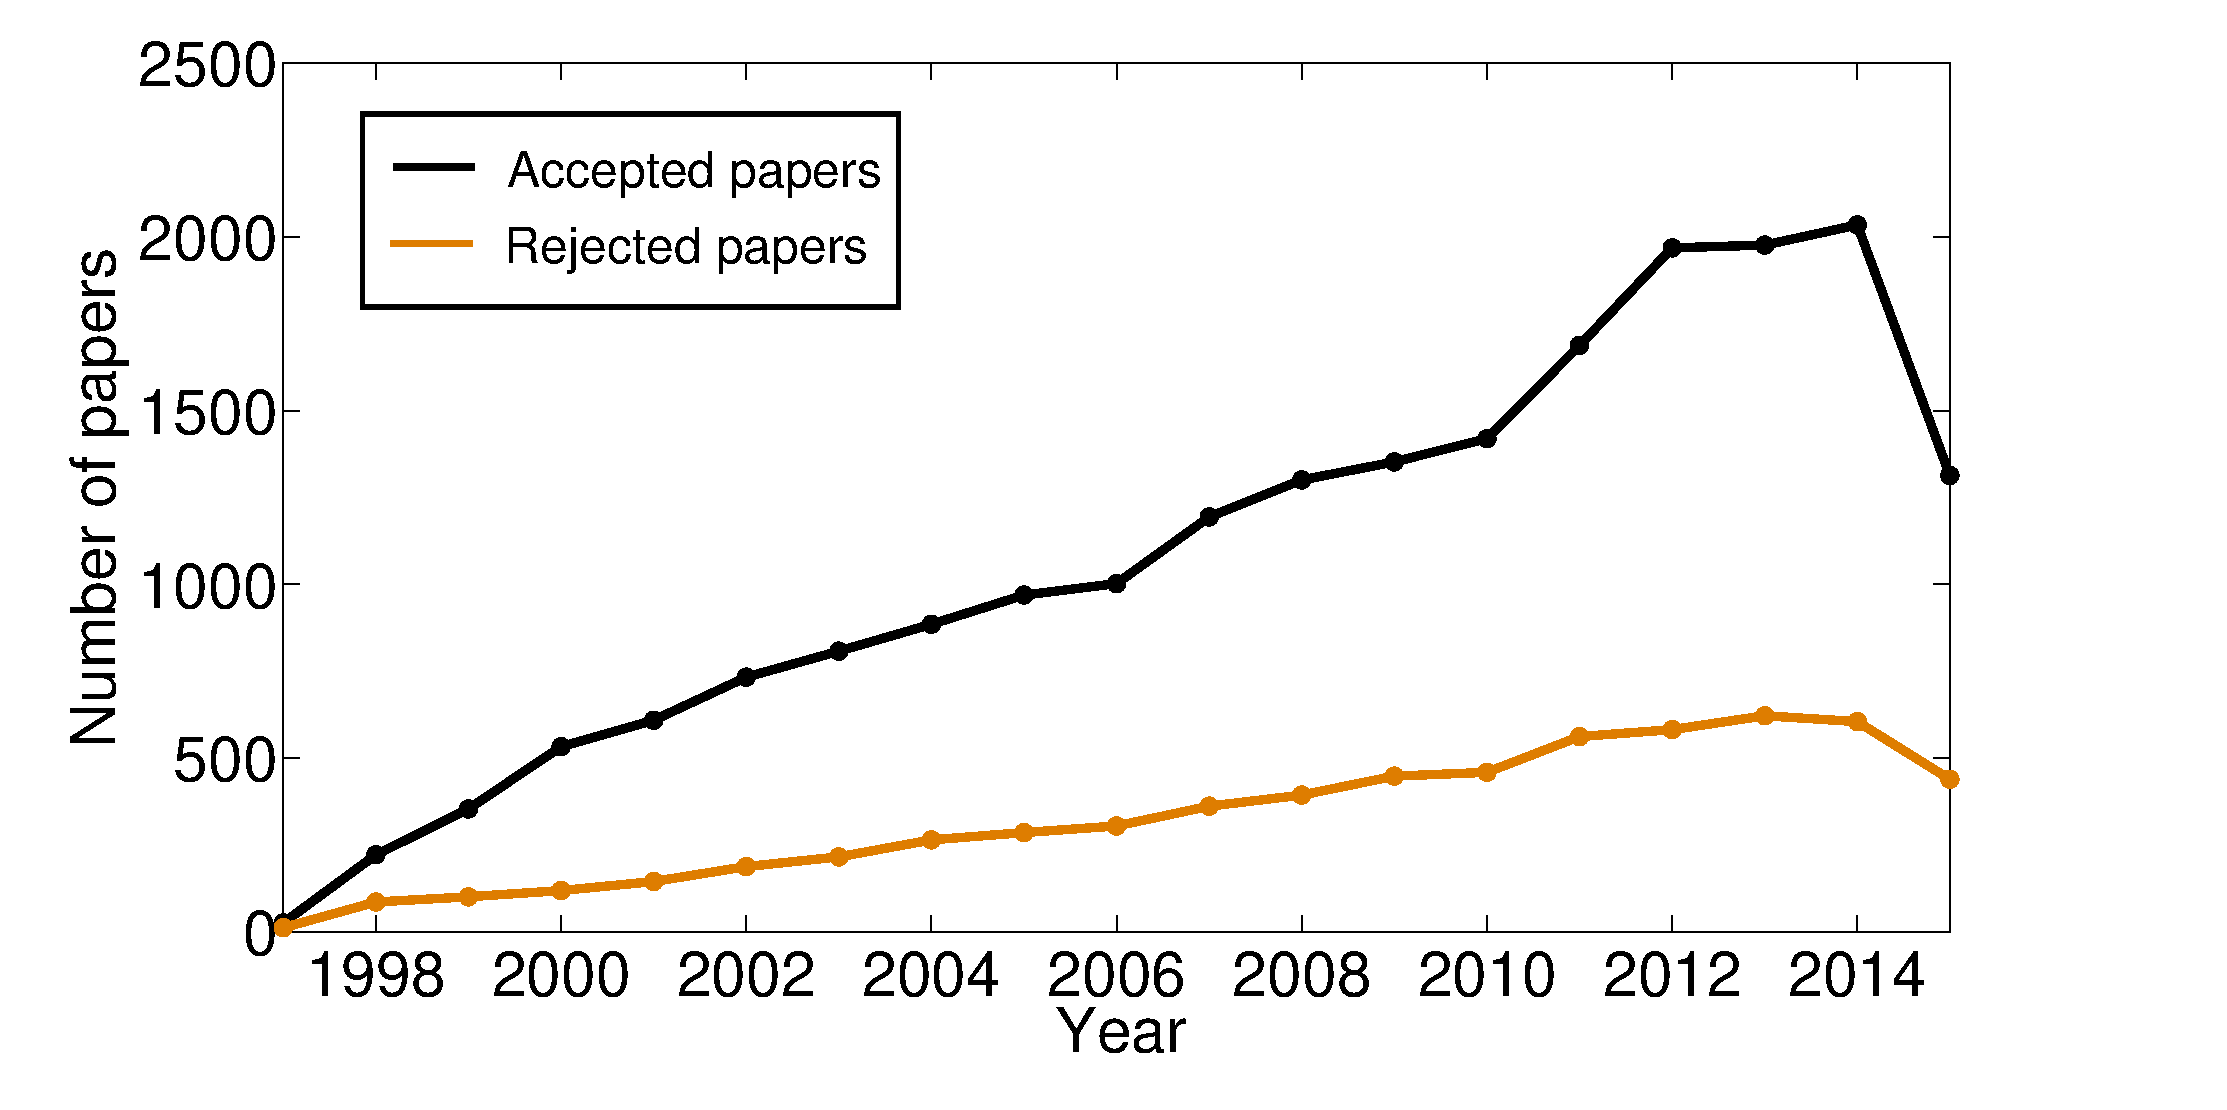
\includegraphics[scale=0.22]{figures/paper_year_dis}
%\caption{\label{fig1} Number of accepted and rejected papers per year from 1997-2015.}
%\end{figure}
%The dataset only offers the meta information for papers submitted to JHEP. So 
We further queried the {\em Inspire} \footnote{https://inspirehep.net/} database to obtain the meta information of the papers (not published/rejected in JHEP). Using this information we created a citation profile for each paper i.e., citations received by the paper per year from the year of its publication. Garfield et. al. ~\cite{garfield1999journal} had noted that most papers receive the bulk of their citations within the first three years of publication. Moreover it is known that old papers generally have more citations, as the paper had more time to accumulate the citations. Thus to account for this effect,  we  calculated total citations received by each paper in the first three years from its year of publication (e.g., for a paper published in 2007 we consider the citations received by it till 2010). For the rest of this article, by citation of a paper we refer to the number of citations it received in the first three years from the year of its publication and we only consider the papers published between 1997 to 2012 for our experiments. 
%To obtain the necessary information for the rejected papers we further queried the ``Inspire'' search engine by their corresponding arXiv\footnote{\url{http://arxiv.org/}} ids. \\
Some general properties of the whole dataset are summarized below - \\
%(i) Increasing trend in the number of submissions except for the year 2015 for which the data is incomplete (Figure \ref{fig1}).
%(ii) Citation distribution of the accepted as well as the rejected papers follow power-law behavior (Figure \ref{fig2}).
(i) Number of unique editors in the dataset is 95 while the number of reviewers is 4035.\\ 
(ii) There are $15127$ unique authors in the dataset and of those $12434$ have at least one accepted paper.\\
(iii) Average number of submissions per author is $5.18$ while the average number of authors per paper is 2.87.\\
%We note certain general statistic pertaining to the dataset in Table \ref{tab1}.
(iv) Average number of reviews for accepted and rejected are $1.76$ and $1.35$ respectively.\\
(v) Average number of assignments per editor is $298.28$ while per reviewer it is $7.52$.\\

%\noindent
\section{Anomalous behavior}
\label{anomalies}
In the peer-review process each submission is assigned to an editor who in turn assigns one or more reviewers with the task of judging the quality of the contributions of the submitted paper. The reviewer submits a report to the editor who in turn takes the final decision as to accept or reject the paper based on the report. Therefore, the editors and the reviewers are the two important entities of the peer-review system and they are mainly responsible for ensuring that flawed research does not get into the literature while at the same time correctly identify impactful contributions for publication.  
 So in our setting we define the following two cases to be anomalous - \\
(i) Accepted papers having low citation (research wrongly judged as impactful). \\
(ii) Rejected papers having high citation (quality research wrongly judged as flawed). \\
In this section we look into the anomalous behavior of the two important entities of the peer-review process: (i) the editors and (ii) the reviewers.
\fi

\section{Anomalous behavior}
\label{anomalies}
In the peer-review process each submission is assigned to an editor who in turn assigns one or more reviewers with the task of judging the quality of the contributions of the submitted paper. The reviewer submits a report to the editor who in turn takes the final decision as to accept or reject the paper based on the report. Therefore, the editors and the reviewers are the two important entities of the peer-review system and they are mainly responsible for ensuring that flawed research does not get into the literature while at the same time correctly identify impactful contributions for publication.  
 So in our setting we define the following two cases to be anomalous - \\
(i) Accepted papers having low citation (research wrongly judged as impactful). \\
(ii) Rejected papers having high citation (quality research wrongly judged as flawed). \\
In this section we look into the anomalous behavior of the two important entities of the peer-review process: (i) the editors and (ii) the reviewers.

%\noindent
\subsection{Editor}
\label{editor}   

\begin{figure}
\centering
\includegraphics*[width=.8\textwidth]{./texfiles/Chapter_4/cikm/figures/editor_all.eps}
\caption{\label{fig3}(a) Median Average citation (MAC) versus $MEAT$. $MEAT$ values are bucketed into 12 bins of equal size with range(1, 498.8).(b) MAC versus $SRI$ and (c) MAC versus $RADI$. For both (b) and (c), the x-axis values are bucketed by values corresponding to ($\geq$ 0 and $<$ 0.1), ($\geq$ 0.1 and $<$ 0.2) and so on.}
\end{figure}

\begin{figure}[!ht]
\centering
\includegraphics[scale=0.3]{./texfiles/Chapter_4/cikm/figures/RDI_RDI_diversity.eps}
\caption{\label{fig_sri} (a) Median Average citation versus $SRI$. $SRI$ values are bucketed by values corresponding to ($\geq$ 0 and $<$ 0.1), ($\geq$ 0.1 and $<$ 0.2) and so on. (b) $RDI$ versus number of declines. Increasing trend indicates higher the $RDI$, higher is the number of declines.}
\vspace{3mm}
\end{figure}

\begin{figure}[!ht]
\centering
\includegraphics*[width=0.8\textwidth]{./texfiles/Chapter_4/cikm/figures/reviewer_all.eps}
\caption{\label{fig5}(a) Median Average citation (MAC) versus $MRAT$. $MRAT$ values are bucketed into 20 buckets of equal size with range(1,498.8),(b) MAC versus $MRSD$ (c) MAC versus $TDI$, (d) MAC versus $EDI$, (e) MAC versus $MTD$ and (f) MAC versus $AR$. For both (c),(d) and (e), the x-axis values are bucketed by values corresponding to ($\geq$ 0 and $<$ 0.1), ($\geq$ 0.1 and $<$ 0.2) and so on. For (b) and (f) values (x-axis) are divided into 10 buckets of equal size.}
\end{figure}

We begin by analyzing the anomalous behavior of the editors. We define the behavior of an editor to be anomalous if the papers assigned to her are on average cited less when accepted or are cited more when rejected. In specific, we investigate different factors related to the editor that can lead to such anomaly.
\subsubsection{Mean Editor Assignment Time (MEAT)}
For each editor we obtain the time span (in days) between any two consecutive assignments and calculate the average time span between the two assignments. 
%The main objective is to check whether an editor who is assigned less frequently does a better job than an editor who is assigned more frequently. 
Formally, we define for editor $i$, $MEAT_{i}$ as
\begin{center}
$MEAT_{i}=\frac{1}{n-1}\sum (\delta_{j+1} - \delta_{j})$
\end{center}
where $n$ is the total number of assignments to the editor $i$ and $\delta_{j}$ is the date of the $j$$^\textrm{th}$ assignment. 
In figure~\ref{fig3}(a) we bin the editors based on the $MEAT$ and calculate the median average citation of the papers assigned to the editors in each bin. 
{We observe that for accepted papers very low or very high $MEAT$ values lead to lower citations. An exact opposite behavior is observed for rejected papers. 
This indicates that editors who are assigned time and again (low $MEAT$) or rarely (high $MEAT$) often fail to judge the quality of the papers assigned to them.} 
%Citation increases as $MEAT$ value increases which is then followed by decrease {\bf Not Clear} indicating that editors who are assigned very less frequently are also anomalous. 

\subsubsection{Self Review Index (SRI)}

%In many cases an editor assigns himself as a reviewer instead of assigning a different referee. While in some of these cases she could not find a reviewer (the reviewer declined), in many other cases she did not try to find a reviewer in the first place. 
{\bf Self Review Index (SRI)} measures the fraction of papers for which the editor assigned herself as the reviewer. 
Formally, for an editor $i$, we define $SRI_{i}$ as 
\begin{center}
$SRI_{i}=\frac{\varrho_{i}}{\rho_{i}}$
\end{center}
where $\rho_{i}$ is the number of papers $i$ was assigned as editor while $\varrho_{i}$ is the number of papers $i$ assigned herself as reviewer. We observe that with increasing values of $SRI$ the median average citation for accepted papers decreases while that for rejected papers increases (refer to figure \ref{fig3}(b)). 

\subsubsection{Referee-Author pair Diversity Index (RADI)}

We observe that editors in numerous cases assign papers from a certain author to only a certain reviewer. To investigate whether this allows for less impactful research from this author getting accepted, we define a metric which we call {\bf Referee-Author pair Diversity Index (RADI)}. Formally we define for editor $i$, the $RADI_{i}$ score as 

\begin{center}
$RADI_{i}=-\sum \limits_{j,k} p_{j,k} \log p_{j,k}$
\end{center}

where $p_{j,k}$ denotes the proportion of times a paper from author $k$ was assigned to reviewer $j$ by the editor $i$. In figure~\ref{fig3}(c) we bin the editors based on the $RADI$ and calculate the median average citation of the papers assigned to the editors in each bin. We observe that more the diversity score higher is the citation of the accepted papers and correspondingly lower is the citation of the rejected papers.


%[{\color{red}{\bf Check the last line; I have changed it. What you wrote earlier was not correct.}}]

\subsubsection{Referee Diversity Index (RDI)}
As a following step, we check whether an editor always chooses from a fixed set of reviewers or a diverse set of reviewers while making a paper assignment and, more importantly, does this influence the performance of the editor in terms of the impact of the reviewed paper. We define for each editor($i$) a metric called {\bf Referee Diversity Index ($RDI_{i}$)} as -  
%which assigns a diversity score for each reviewer depending on whether she selects from a diverse set of reviewers or a small fixed set while assigning. Formally for an editor $i$, $RDI_i$ is defined as
\begin{center}
$RDI_{i}=-\sum \limits_{j} p_{j}\log p_{j}$
\end{center}
where $p_{j}$ denotes the proportion of times reviewer $j$ was assigned a paper by editor $i$. More diverse the set of reviewers higher is the score. In figure~\ref{fig3}(b) we bin the editors based on the $RDI$ and calculate the median average citation of the papers assigned to the editors in each bin. We observe that more the diversity score, higher is the citation of the accepted papers and correspondingly lower is the citation of the rejected papers.

A summary statistic of all the above factors that may be used to identify anomalous editors are noted in Table~\ref{summary_stat}.

%\subsubsection*{Pathological cases}
The dataset allows us to find out the cases when the reviewer declined to review a paper on being assigned by an editor. We observe that editors with high $RDI$ are also declined more often. In figure~\ref{fig_sri}(b) we plot $RDI$ value and the number of declines for each editor. An increasing trend indicates that more diversely the editor tries to select reviewers more she gets declined by the reviewers. This in many cases may force the editor to be less proactive and always select from a specific set of `reliable' referees.  

%\subsubsection*{Pathological cases}

%We further looked into some pathological cases which are summarized below - \\
%(i) There are {\bf 1598} submissions which were initially rejected and then successfully appealed by the authors for reconsideration. {\bf 48.72\%} of these were finally accepted, while rest of them were either rejected or withdrawn by the authors. An important observation is that in {\bf 19.8\%} of the cases the paper was again assigned the same editor while for the rest a new editor was assigned. Another surprising observation is that in the {\bf 45.6\%} of the cases where the paper was finally accepted, it was assigned to a specific editor.\\
%(ii) There are {\bf 4006} papers that were declined at least once by a reviewer before being reviewed. We observed that the papers which were declined more than once tend to be low cited on average.
%\begin{figure}
%\centering
%\includegraphics[scale=0.23]{figures/div_decline.eps}
%\caption{\label{fig4} $RDI$ versus number of declines. Increasing trend indicates higher the $RDI$, higher is the number of declines.}
%\end{figure}

\subsection{Editor}
\label{editor}   

\begin{figure}
\centering
\includegraphics[width=.9\textwidth]{./texfiles/Chapter_4/cikm/figures/editor_all.eps}
\caption{\label{fig3}(a) Median Average citation (MAC) versus $MEAT$. $MEAT$ values are bucketed into 12 bins of equal size with range(1, 498.8).(b) MAC versus $SRI$ and (c) MAC versus $RADI$. For both (b) and (c), the x-axis values are bucketed by values corresponding to ($\geq$ 0 and $<$ 0.1), ($\geq$ 0.1 and $<$ 0.2) and so on.}
\end{figure}

\begin{figure}[!ht]
\centering
\includegraphics[scale=0.4]{./texfiles/Chapter_4/cikm/figures/RDI_RDI_diversity.eps}
\caption{\label{fig_sri} (a) Median Average citation versus $SRI$. $SRI$ values are bucketed by values corresponding to ($\geq$ 0 and $<$ 0.1), ($\geq$ 0.1 and $<$ 0.2) and so on. (b) $RDI$ versus number of declines. Increasing trend indicates higher the $RDI$, higher is the number of declines.}
\end{figure}

\begin{figure}[!ht]
\centering
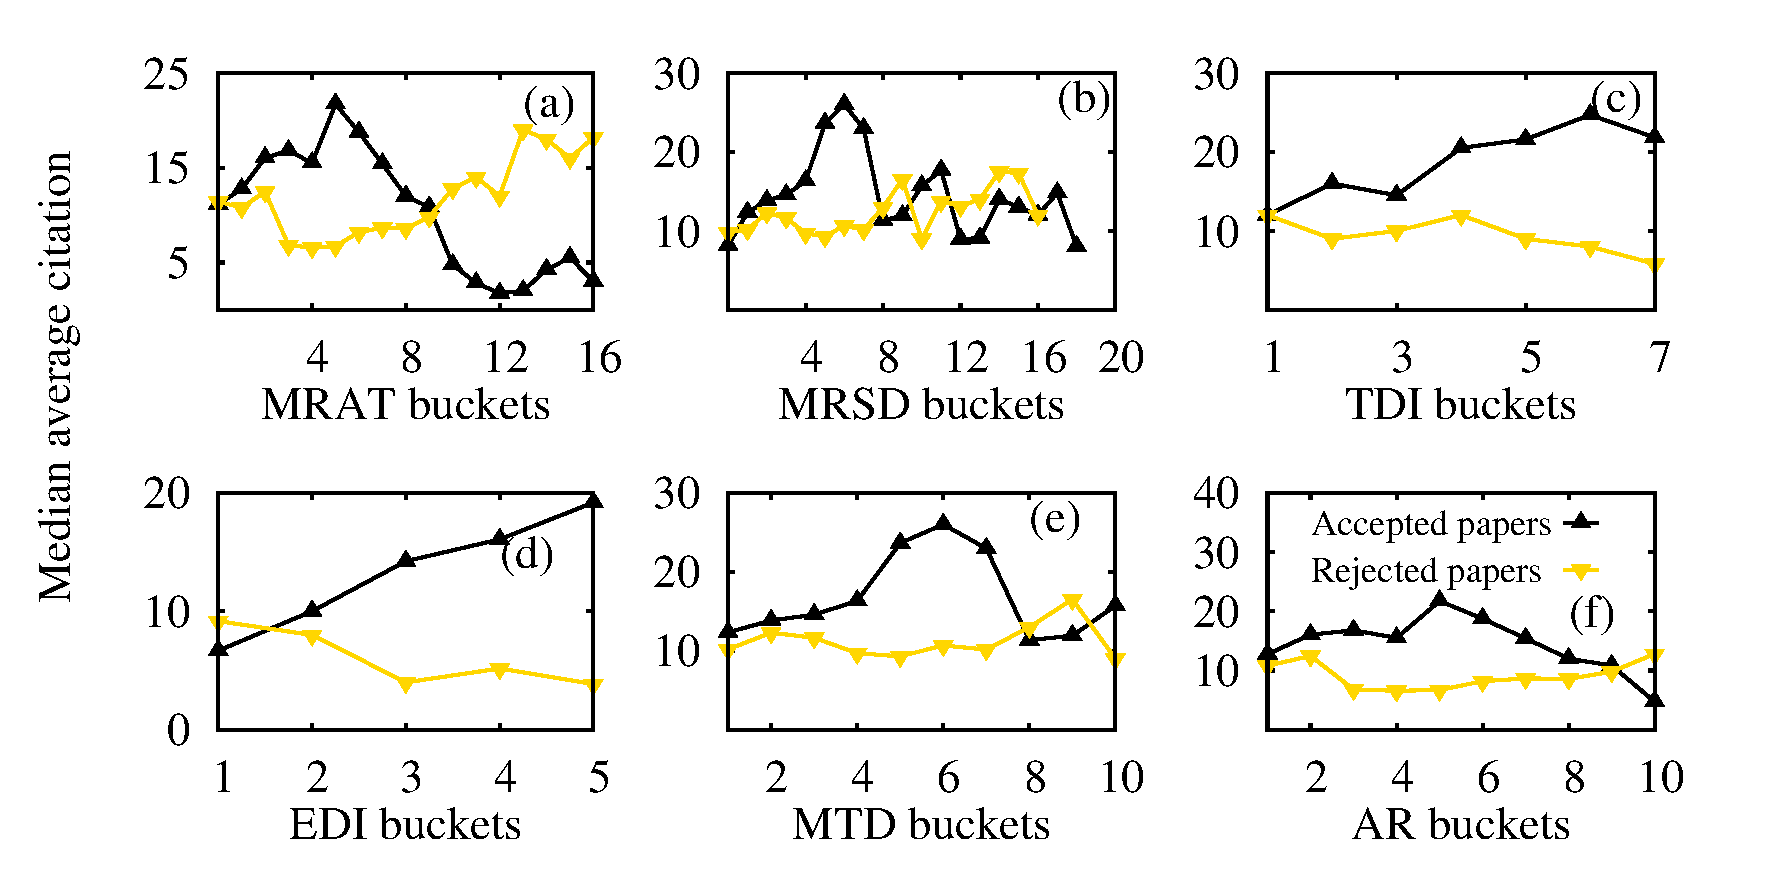
\includegraphics[width=0.9\textwidth]{./texfiles/Chapter_4/cikm/figures/reviewer_all.eps}
\caption{\label{fig5}(a) Median Average citation (MAC) versus $MRAT$. $MRAT$ values are bucketed into 20 buckets of equal size with range(1,498.8),(b) MAC versus $MRSD$ (c) MAC versus $TDI$, (d) MAC versus $EDI$, (e) MAC versus $MTD$ and (f) MAC versus $AR$. For both (c),(d) and (e), the x-axis values are bucketed by values corresponding to ($\geq$ 0 and $<$ 0.1), ($\geq$ 0.1 and $<$ 0.2) and so on. For (b) and (f) values (x-axis) are divided into 10 buckets of equal size.}
\end{figure}

We begin by analyzing the anomalous behavior of the editors. We define the behavior of an editor to be anomalous if the papers assigned to her are on average cited less when accepted or are cited more when rejected. In specific, we investigate different factors related to the editor that can lead to such anomaly.
\subsubsection{Mean Editor Assignment Time (MEAT)}
For each editor we obtain the time span (in days) between any two consecutive assignments and calculate the average time span between the two assignments. 
%The main objective is to check whether an editor who is assigned less frequently does a better job than an editor who is assigned more frequently. 
Formally, we define for editor $i$, $MEAT_{i}$ as
\begin{center}
$MEAT_{i}=\frac{1}{n-1}\sum (\delta_{j+1} - \delta_{j})$
\end{center}
where $n$ is the total number of assignments to the editor $i$ and $\delta_{j}$ is the date of the $j$$^\textrm{th}$ assignment. 
In figure~\ref{fig3}(a) we bin the editors based on the $MEAT$ and calculate the median average citation of the papers assigned to the editors in each bin. 
{We observe that for accepted papers very low or very high $MEAT$ values lead to lower citations. An exact opposite behavior is observed for rejected papers. 
This indicates that editors who are assigned time and again (low $MEAT$) or rarely (high $MEAT$) often fail to judge the quality of the papers assigned to them.} 
%Citation increases as $MEAT$ value increases which is then followed by decrease {\bf Not Clear} indicating that editors who are assigned very less frequently are also anomalous. 

\subsubsection{Self Review Index (SRI)}

%In many cases an editor assigns himself as a reviewer instead of assigning a different referee. While in some of these cases she could not find a reviewer (the reviewer declined), in many other cases she did not try to find a reviewer in the first place. 
{\bf Self Review Index (SRI)} measures the fraction of papers for which the editor assigned herself as the reviewer. 
Formally, for an editor $i$, we define $SRI_{i}$ as 
\begin{center}
$SRI_{i}=\frac{\varrho_{i}}{\rho_{i}}$
\end{center}
where $\rho_{i}$ is the number of papers $i$ was assigned as editor while $\varrho_{i}$ is the number of papers $i$ assigned herself as reviewer. We observe that with increasing values of $SRI$ the median average citation for accepted papers decreases while that for rejected papers increases (refer to figure \ref{fig3}(b)). 

\subsubsection{Referee-Author pair Diversity Index (RADI)}

We observe that editors in numerous cases assign papers from a certain author to only a certain reviewer. To investigate whether this allows for less impactful research from this author getting accepted, we define a metric which we call {\bf Referee-Author pair Diversity Index (RADI)}. Formally we define for editor $i$, the $RADI_{i}$ score as 

\begin{center}
$RADI_{i}=-\sum \limits_{j,k} p_{j,k} \log p_{j,k}$
\end{center}

where $p_{j,k}$ denotes the proportion of times a paper from author $k$ was assigned to reviewer $j$ by the editor $i$. In figure~\ref{fig3}(c) we bin the editors based on the $RADI$ and calculate the median average citation of the papers assigned to the editors in each bin. We observe that more the diversity score higher is the citation of the accepted papers and correspondingly lower is the citation of the rejected papers.


%[{\color{red}{\bf Check the last line; I have changed it. What you wrote earlier was not correct.}}]

\subsubsection{Referee Diversity Index (RDI)}
As a following step, we check whether an editor always chooses from a fixed set of reviewers or a diverse set of reviewers while making a paper assignment and, more importantly, does this influence the performance of the editor in terms of the impact of the reviewed paper. We define for each editor($i$) a metric called {\bf Referee Diversity Index ($RDI_{i}$)} as -  
%which assigns a diversity score for each reviewer depending on whether she selects from a diverse set of reviewers or a small fixed set while assigning. Formally for an editor $i$, $RDI_i$ is defined as
\begin{center}
$RDI_{i}=-\sum \limits_{j} p_{j}\log p_{j}$
\end{center}
where $p_{j}$ denotes the proportion of times reviewer $j$ was assigned a paper by editor $i$. More diverse the set of reviewers higher is the score. In figure~\ref{fig3}(b) we bin the editors based on the $RDI$ and calculate the median average citation of the papers assigned to the editors in each bin. We observe that more the diversity score, higher is the citation of the accepted papers and correspondingly lower is the citation of the rejected papers.

A summary statistic of all the above factors that may be used to identify anomalous editors are noted in Table~\ref{summary_stat}.

%\subsubsection*{Pathological cases}
The dataset allows us to find out the cases when the reviewer declined to review a paper on being assigned by an editor. We observe that editors with high $RDI$ are also declined more often. In figure~\ref{fig_sri}(b) we plot $RDI$ value and the number of declines for each editor. An increasing trend indicates that more diversely the editor tries to select reviewers more she gets declined by the reviewers. This in many cases may force the editor to be less proactive and always select from a specific set of `reliable' referees.  


%\noindent
\subsection{Analyzing reviewer tendencies}
\label{reviewer}
%\mycheckng{What percentage of reviewers are anomalous}
Reviewers are assigned with the responsibility of judging the quality of a submitted paper and hence their knowledge and training is highly critical. 
In fact, the decision of acceptance or rejection of a paper depends on the reviewer's perception of the paper. 

%\begin{figure}
% \centering
% \includegraphics[scale = 0.26]{figures/reviewer.eps}
% \caption{\label{reviewer} Cumulative distribution function of fraction of cases a reviewer was a part of a multi-referee system across all the reviewers
% for both JHEP and JSTAT datasets.}
%\end{figure}



%We calculate for each reviewer the fraction of cases where he is a part of a multi-referee set among his total assignments and plot the 
%cumulative distribution function of this fraction in figure~\ref{reviewer} for both JHEP and JSTAT datasets. The figure clearly indicates 
%that for JHEP the reviewers are mostly part of a single-referee set up while for JSTAT, the reviewers are part of a multi-referee set up in many more cases. 

% \begin{figure} 
%  \centering
%  \includegraphics[scale = 0.26]{figures/ed_ref_comb.eps}
%  \caption{\label{reviewer} Cumulative distribution function of the fraction of cases a reviewer is a part of a multi-referee system across all the reviewers for JHEP and JSTAT datasets.}\end{figure}
\begin{figure}
 \centering
 \includegraphics[scale = 0.3]{./texfiles/Chapter_4/cikm_17/figures/citation_delay_acpt_ratio_jhep.eps}
 \caption{\label{a_d_jhep} Mean citation versus (a) accept ratio (b) assignment delay buckets for the JHEP dataset. 
 Note that the papers are segregated into accept ratio/delay bins and the mean citation is calculated for each bin. 
 Typical bin sizes for accept ratio are $<0.1$,$(\geq 0.1$ and $<0.2)$ and so on while for delay the sizes are $<100$, $(\geq 100$ and $< 200)$ and so on.\vspace{4mm}}
\vspace{3mm}
 \end{figure}

%We further leverage the technique introduced in~\cite{sikdar2016anomalies} and identify the set of under-performing
% reviewers for both the datasets. 
% \mycheck{put in the definition of underperforming/anomalous-----}
In the last section we defined a referee/editor to be anomalous (under-performing) if - \\
(i) papers accepted by him/her have low citation (research wrongly judged to be impactful)\\
(ii) papers rejected by him/her have high citation (quality research wrongly judged as flawed)\\
%In fact, the authors propose a method for identifying under-performing (anomalous) referees/editors. Leveraging on the same method we observe that  
% the proportion of referees classified as under-performing are approximately $26\%$ and $21\%$ respectively for JHEP and JSTAT datasets.
%The authors hypothesize that accepted papers receiving low citation as well as rejected papers receiving high citations are anomalous cases as 
%ideally they should have been respectively rejected and accepted.  
We make the following general observations - \\
(i) If we consider all the cases where an under-performing editor assigned multiple reviewers for a submission, in $69.8\%$ cases 
at least one of them was under-performing. This indicates that unless the reviewers are selected carefully, chances are it might lead to wrong judgment.\\
(ii) Under-performing reviewers when part of a multi-referee system tend to do a better judgment as compared to cases when they serve as single reviewers.
This is illustrated by the fact that average citation of the accepted  papers reviewed by multiple reviewers with at least one under-performing reviewer ($32.4$) 
is more compared to that of the papers reviewed by a single anomalous reviewer ($18.2$) across the two datasets.
%\vspace{-4mm}
\subsubsection{Factors determining performance of the referees}
We next look into factors that could be used to quantify the performance of the reviewers. The quantification can be used as a 
fitness value for assignment of a new submission (we use these to calculate these quantities in a later section to develop a scheme for automatic referee group selection). 
Given a submission, we identify two factors that are indicative of reviewer fitness (i) accept ratio and (ii) time since the last assignment.\\
\noindent(i) \textit{Accept ratio}: Given a submission, we consider for each reviewer ($i$) the fraction of papers (s)he has accepted at the time of submission. 
We denote this by $a_i$. To show that it is indeed an indicator we consider all the accepted and the rejected papers as well as their assigned reviewers. 
We then calculate the accept ratio of the assigned reviewers and compare them against the citations received by each of them. 
In figures~\ref{a_d_jhep}(a) (JHEP) and~\ref{a_d_jstat}(a) (JSTAT) we plot the accept ratio against the citations received by the accepted as well as the rejected papers. 
Note that we bin the papers based on the accept ratio and calculate the average citation in each case. The typical bin sizes are $\leq 0.1$, $(> 0.1$ and $\leq 0.2)$ and so on. 
We hence obtain $10$ such bins numbered 1-10. 
In case of multi-referee papers the average accept ratio of the reviewers is considered. We observe that for both the datasets very high accept ratio or a very low accept 
ratio might lead to wrong judgment. \\ 
\noindent(ii) \textit{Time since last assignment}: Given a submission and its corresponding submission date we calculate for each reviewer ($i$) the time (in days) between the 
last review assignment date and the submission date (denoted by $d_i$). To illustrate the rationale, we again consider all the accepted and the rejected papers and calculate 
the delay for the assigned reviewers. We again bin the delay values and calculate the average citation (refer to figures~\ref{a_d_jhep}(b) and~\ref{a_d_jstat}(b)). Typical bin 
sizes are $\leq 100$, $(> 100$ and $\leq 200)$ and so on (10 such bins are obtained numbered 1-10). We observe that the reviewers who are assigned very close to their last 
assignment or those who have not been assigned for a long time often fail to correctly judge the quality of the paper correctly as the papers accepted by them are cited less 
on average while those rejected are cited more. 


% \begin{figure}
%  \centering
%  \includegraphics[scale = 0.26]{figures/citation_delay_acpt_ratio_jhep.eps}
%  \caption{\label{a_d_jhep} Mean citation versus (a) accept ratio (b) assignment delay buckets for the JHEP dataset. 
%  Note that the papers are segregated into accept ratio/delay bins and the mean citation is calculated for each bin. 
%  Typical bin sizes for accept ratio are $<0.1$,$(\geq 0.1$ and $<0.2)$ and so on while for delay the sizes are $<100$, $(\geq 100$ and $< 200)$ and so on.}
% \end{figure}

\begin{figure}
 \centering
 \includegraphics[scale = 0.3]{./texfiles/Chapter_4/cikm_17/figures/citation_delay_acpt_ratio_jstat.eps}
 \caption{\label{a_d_jstat} Mean citation versus (a) accept ratio (b) assignment delay buckets for JSTAT dataset. Note that the papers are 
 segregated into accept ratio/delay bins and the mean citation is calculated for each bin. Bin sizes are same as figure \ref{a_d_jhep}.\vspace{4mm}}
\vspace{3mm}
 \end{figure}



\subsubsection{Action with under-performing reviewers}
A naive solution could be to not assign the under-performing reviewers and only assign the best performing ones, but this is not always feasible 
since the number of referees is limited and they often decline assignments. Hence a better solution would be to group them such that the overall performance improves. 
To this aim, we first divide the reviewers into 3 classes separately for accept ratio and time 
since last assignment. A reviewer $i$ with accept ratio $a_i < 0.3$ is assigned ``Low'' (L), with $0.3 \leq a_i < 0.6$ is assigned ``Medium'' (M) and with $a_i \geq 0.6$ is 
assigned ``High'' (H). Note that reviewers in M were the best performing referees (refer to figures \ref{a_d_jhep}(a) and \ref{a_d_jstat}(a)). Each multi-refereed paper 
(by exactly 2 referees) is classified into one of the six classes (LL, MM, HH, LH, MH, LH) based on the class of each referee and the average citation of the papers in each 
class is noted (figure \ref{ref_perf}(a)). We observe that when both the referees belong to the M class (MM) the performance is naturally well. More importantly, reviewers in L and H class 
perform better when paired with a referee from M class (even better than MM). On repeating the same experiment with time since last assignment, 
we observe a similar trend (figure \ref{ref_perf}(b)) with MM class performing the best followed by MH and LM.  
Note that in this case reviewers with $d_i < 100$ are assigned class L, with $100 \leq d_i < 300$ are assigned M and rest are assigned H. 
%This indicates that grouping 
%reviewers while assigning multiple referees for a 
%submission is highly critical toward improving the effectiveness of the system. 
%We further look into the proportion of discordant cases for each reviewer combination. 
More importantly the discordant cases mostly occur for 
class combinations LL, HH and LH (refer to table \ref{tab:dis}). In fact, MM has the least proportion of discordant cases. 
This further indicates the correct reviewer grouping is critical in curtailing the discordant cases which is one of the prime reasons behind the multi-reviewer system failing. 
Note that the above results are obtained for JHEP dataset and a similar pattern is observed 
for JSTAT as well.

\begin{figure}
 \centering
 \includegraphics[scale = 0.3]{./texfiles/Chapter_4/cikm_17/figures/ref_performance.eps}
 \caption{\label{ref_perf} Mean citation for papers belonging particular class combination with respect to (a) accept ratio (b) time since last assignment. For example LL would represent a paper reviewed by referees both 
 belonging to class L.\vspace{4mm}}
\end{figure}







\medskip


\subsection{Reviewer}
\label{reviewer}

In this section, we investigate anomalous behavior of the referees. Recall that we define the behavior of a reviewer to be anomalous if the papers accepted by her are low cited or the papers rejected by her are highly cited. As in case of the editors, here also we investigate different factors that could be indicative of such anomalous behavior.  

\subsubsection{Mean Reviewer Assignment Time (MRAT)}

%For each individual reviewer we find the time difference (in days) between two consecutive assignments. Note that we do not consider the cases where the reviewer was assigned but she declined to review it.
This is essentially same as MEAT. For a reviewer $i$, we define $MRAT_{i}$ as
\begin{center}
$MRAT_{i}=\frac{1}{n-1}\sum (\delta_{j+1} - \delta_{j})$
\end{center}
\noindent where $n$ is the total number of assignments of reviewer $i$ and $\delta_{j}$ is the date of the $j^\textrm{th}$ assignment. In figure~\ref{fig5}(a) we plot $MRAT$ (binned) and median average citation of the papers reviewed for each reviewer. We observe that papers reviewed by reviewers with low $MRAT$ (high frequency of assignment) tend to be cited less and increases as $MRAT$ increases. This is followed by again a steep decrease in citation. This indicates that the reviewers assigned very frequently are often less reliable while those assigned only occasionally are also not likely to correctly judge the quality of the paper.  

\subsubsection{Mean Report Sending Delay (MRSD)}

We argue that the time taken by a reviewer to send back the review report could be an indicator of his performance. If a reviewer on average sends back the review very quickly it is highly likely that the review was done in a hurry. Similarly, if the report was sent after being reminded by the editor numerous times, it is also highly likely the review report could be anomalous. For a reviewer we calculate the time delay between the date of her assignment and the date she sent back the report for each of her assignments. To measure $MRSD$ we calculate the mean value of all the delays. Note that we do not consider the assignments which the reviewer declined. Formally, for a reviewer $i$, we define $MRSD_{i}$ as 

\begin{center}
$MRSD_{i}=\frac{1}{n}\sum(\delta_{i}-\Delta_{i})$
\end{center}

where $n$ is the total number of assignments, $\Delta_{i}$ is the date of assignment and $\delta_{i}$ is the date when the report was received by the editor. On plotting against median average citation we observe a similar trend as was observed in case of $MRAT$ (refer to figure~\ref{fig5}(b)). Papers reviewed by reviewers with low $MRSD$ value are often less cited, indicating that reviewers sending back their report very quickly often do it in a hurry and fail to correctly judge the quality of the paper while those taking very long to send report are prone to failure as well. 

\subsubsection{Topic Diversity Index (TDI)}

JHEP associates with each submission a set of keywords which roughly indicates the domain of the work. We use these associated keywords as a proxy for topic. For each reviewer, we segregate all the keywords of the papers reviewed by her which we call the keyword corpus for the reviewer. Formally for a reviewer $i$, we define $TDI_{i}$ as 

\begin{center}
$TDI_{i}=-\sum \limits_{j} p_{j}\log p_{j}$
\end{center}

\noindent where $p_{j}$ is the proportion of keyword $j$ in the keyword corpus for reviewer $i$. We segregate the reviewers based on the diversity score and calculate the median average citation of the papers reviewed by them. We observe that the median average citation %[{\color{red}{\bf Why introduce this acronym here? Use it from the first time it has been invoked.}}] 
for reviewers with low $TDI$ are low mainly because the number of papers reviewed by them are also less. The value increases with  increasing $TDI$ (refer to figure~\ref{fig5}(c)). The reviewers with low $TDI$ are often the ones who have reviewed a very small number of papers while the reviewers with high $TDI$ are mostly assigned papers by a large number of editors. 
 
 
 
\subsubsection{Editor Diversity Index (EDI)}

Reviewers could be selected for review by a large set of editors or could only be selected by a single or a small set of editors. We check whether a reviewer selected by many editors is more reliable compared to one who is selected by a single or a very small set of editors. To this aim we assign each reviewer a score called Editor Diversity Index, $EDI_{i}$ which is defined as 

\begin{center}
$EDI_{i}=-\sum \limits_{j} p_{j}\log p_{j}$
\end{center}

where $p_{j}$ represents the proportion of times reviewer $i$ was assigned by editor $j$. We segregate the reviewers based on $EDI$ and calculate the median average citation of the papers reviewed by them. We observe that as $EDI$ increases median average citation also increases (refer to figure \ref{fig5}(d)) indicating that reviewers assigned by multiple editors are often more reliable.

\begin{table}[htpb]
\centering
\caption{Features used for detecting anomalies.}
\label{summary_stat}
\small
\begin{tabular}{|l|l|l|l|l|l|l|}
\hline
                        & Factor                                     & Mean & Median & Max & Min & \begin{tabular}[c]{@{}l@{}}St.\\ Dev\end{tabular} \\ \hline
\multirow{3}{*}{Editor} & $MEAT$         & 35.06     &  29.1      &  108.25   &  3.28   & 23.19                                                             \\  
                        & $RDI$              & 6.57     &  6.79      & 8.85    & 0.0    &  1.44                                                            \\ 
                        & $RADI$ & 8.86     & 9.21       & 11.94    & 0.0    &  1.87 
                         \\ 
                        & $SRI$ & 0.28     & 0.25       & 0.85    & 0.0    &  0.19                                                           
                        \\ \hline
\multirow{6}{*}{Reviewer} & $MRAT$       & 363.3     & 193.7       & 5389    & 26.9    & 508.9                                                             \\  
                        & $MRSD$           & 19.28     & 17.50       & 122    & 16.5    &  11.45                                                            \\  
                        & $TDI$                &  4.07    &  3.96      & 8.10    & 1.0    &  1.44                                                            \\  
                        & $EDI$               &  1.12    &   0.91     &  4.58   & 0.0    &   1.19                                                           \\  
                        & $AR$                      &  0.65    &   0.71     &   1.0  & 0.0    &    0.2                                                          \\  
                        & $MTD$                 &   3.86   &  3.12      & 69.0    & 1.0    & 4.96                                                             \\ 
                        & $DFI$                 & 0.19     & 0.12       & 1.0    & 0.0    & 0.30                                                             \\ \hline
                        
\end{tabular}
\end{table} 


\subsubsection{Mean Time to Decline (MTD)}

We further investigated the cases where the reviewer declined the assignment. In specific, we calculated the time delay (in days) 
between the date she was assigned and the date she conveyed her decision of declining to review. For each reviewer we define {\bf Mean Time to Delay}, $MTD_{i}$ as 

\begin{center}
$MTD_{i}= \frac{1}{d}\sum \limits_{j}(\mu_{j} - \Delta_{j})$
\end{center}

where $d$ is the number of assignments that reviewer $i$ declined and $\mu_{j}$ and $\Delta_{j}$ are respectively the date of assignments and date of reply for paper $j$ by reviewer $i$. We segregate the reviewers based on their $MTD$ values and calculate the median average citation. We observe that the reviewers who delay often in reporting their decision to the editor of being unable to review usually tend to fail in judging a paper quality when they do review (refer to figure~\ref{fig5}(f)).

\subsubsection{Acceptance Ratio (AR)}
Acceptance Ratio ($AR$) of a reviewer is defined as the proportion of papers accepted by the reviewer. For a reviewer $i$, $AR_{i}$ is formally defined as 

\begin{center}
$AR_{i}=\frac{a_{i}}{a_{i}+r_{i}}$
\end{center}

\noindent where $a_{i}$ and $r_{i}$ respectively denote the number of papers accepted and rejected by reviewer $i$. We observe that reviewers with high $AR$ often accept  less impactful papers while reviewers with very low $AR$ often fail to identify quality research (refer to figure~\ref{fig5}(e)). Note that the reviewers are segregated based on their respective $AR$ values while the median average citation is calculated. They are segregated into bins based on the $AR$ values where typically the bins are ($\geq$ 0 and $< 0.1$), ($\geq$ 0.1 and $<$ 0.2) and so on.

\begin{figure}
\centering
\includegraphics[scale=0.4]{./texfiles/Chapter_4/cikm/figures/DFI_dec_month.eps}
\caption{\label{fig_dfi}(a) Median Average citation versus $DFI$. $DFI$ values are bucketed by values corresponding to ($\geq$ 0 and $<$ 0.1), ($\geq$ 0.1 and $<$ 0.2) and so on. (b) Number of declines versus the month of the year.}
%\vspace{-.4cm}
\end{figure}
%begin{figure}
%ncludegraphics[scale=0.22]{figures/decline_month.eps}
%aption{\label{fig6} Number of declines versus the month of the year.}
%end{figure}

\subsubsection{Decline Fraction Index (DFI)}

{\bf Decline Fraction Index (DFI)} for a reviewer is the fraction of times she declined to review. For a reviewer $i$, we define $DFI_{i}$ as
\begin{center}
$DFI_{i}=\frac{\vartheta_{i}}{\theta_{i}}$
\end{center}

\noindent where $\theta_{i}$ is the total number of assignments while $\vartheta_{i}$ is the number of times $i$ declined to review. 
In figure \ref{fig_dfi}(a) we plot median average citation versus $DFI$. We observe that for accepted papers the citation is higher for lower $DFI$ values and it drops as $DFI$ increases indicating that reviewers declining too frequently often fail to judge the quality of the paper assigned to them.

A summary statistics of all the above factors that may be used to identify anomalous referees are noted in Table~\ref{summary_stat}.

%\subsubsection*{Pathological Cases}
We further looked into the data and made some interesting observations which are summarized below - \\
(i) A bulk of the instances where a reviewer declined to review occurred in the month of July and August. This is represented in figure~\ref{fig_dfi}(b). This probably relates to the vacation time in the Europe and the US.
(ii) Of the 4035 reviewers 756 of the reviewers have not been assigned a paper for the last two years. On further investigation we observed that among these there are 505 such reviewers who in their immediate last review assignment agreed to review but did not send back the report.


%\noindent
\subsection{Identifying anomalous Editors and Reviewers}
\label{prediction}

%[{\color{red}{\bf Shall ckeck the rest from here after you have a complete version.}}]

In the previous sections we discussed how different factors indicate anomalous behavior of referees and editors. In this section, we check whether we can use them to automatically differentiate between normal and anomalous editors and referees. We propose separate unsupervised models for editors and reviewers.

\begin{figure}
\centering
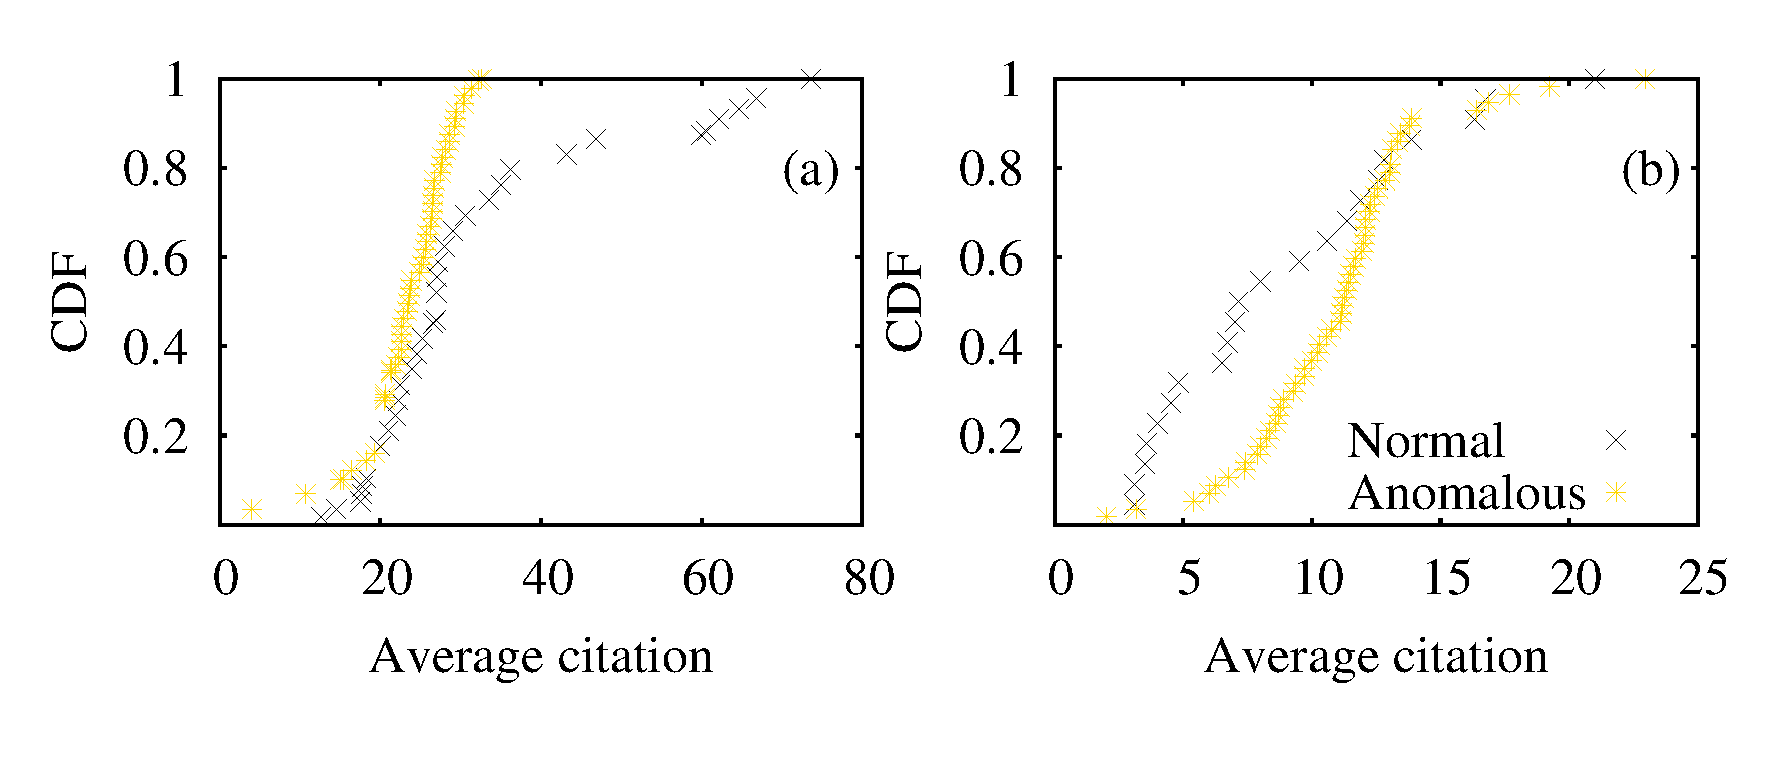
\includegraphics[scale=0.27]{./texfiles/Chapter_4/cikm/figures/editor_all_anom.eps}
\caption{\label{ed_pred}Cumulative distribution function of the average citations for the two sets of editors (anomalous and normal).\vspace{4mm}} 
\end{figure}


\subsubsection{Editors}
For each editor $i$, we measure $MEAT_{i}$, $RDI_{i}$, $RADI_{i}$ and $SRI_{i}$ which form a feature vector. 
%[{\color{red}{\bf Have you not used $SRI$? Why?}}] 
We also consider the editors who were assigned at least 5 papers and accepted at least 1 paper before 2013. 
To detect anomalies we use the 
$k-means$ clustering setting with $k=2$. The two clusters are of sizes 25 and 68 respectively. Clearly this set of 25 editors are the anomalous ones.
In figure \ref{ed_pred} we plot the cumulative distribution of average citation of accepted (figure \ref{ed_pred}(a)) and rejected  (figure \ref{ed_pred}(b)) papers. We observe that citation of accepted papers assigned to anomalous editors are significantly lower while citation of rejected papers are significantly higher compared to those assigned to normal editors.


\subsubsection{Reviewers}

Similarly for each reviewer $i$ we associate a feature vector of size seven consisting of $MRAT_{i}$, $MRSD_{i}$, $TDI_{i}$, $EDI_{i}$, $AR_{i}$, $MTD_{i}$ and $DFI_{i}$. 
%[{\color{red}{\bf Have you not used $DFI$? Why?}}] 
We filter out reviewers who have reviewed at least 5 papers and accepted at least 1 before 2013. This reduces our set of reviewers to 2328. By using $k-means$ clustering ($k=2$), we obtain two clusters of size 339 and 
1999. On plotting cumulative distribution of the average citation for accepted (refer to figure \ref{rev_pred}(a)) and rejected papers (refer to figure \ref{rev_pred}(b)), we observe that the papers accepted by anomalous reviewers are cited significantly lesser while those rejected by them are cited significantly higher compared to the normal referees.

\begin{figure}
\centering
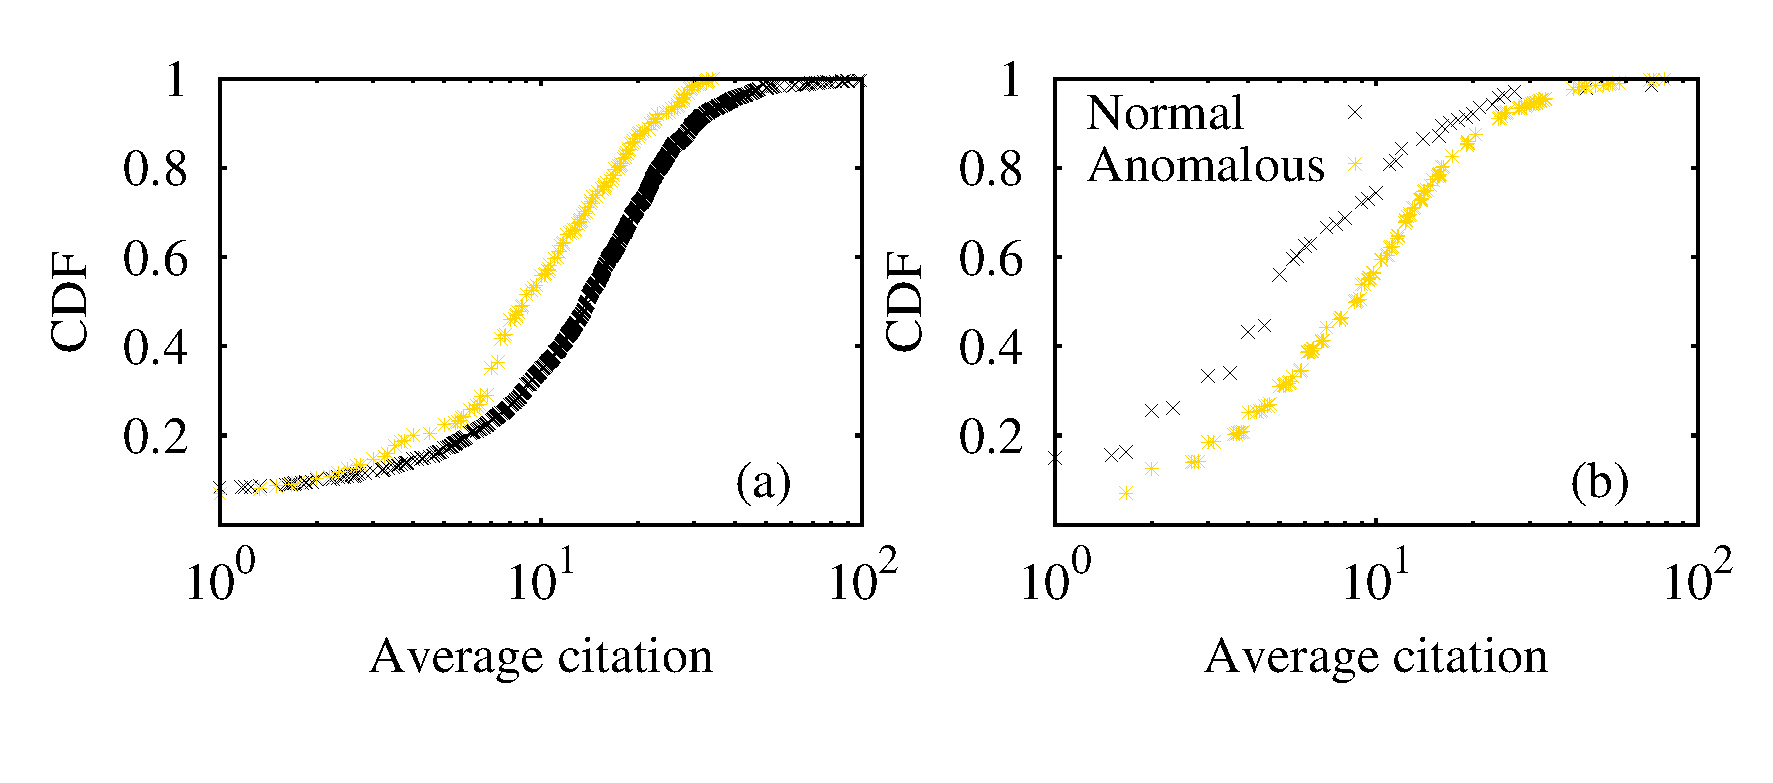
\includegraphics[scale=0.27]{./texfiles/Chapter_4/cikm/figures/reviewer_all_anom.eps}
\caption{\label{rev_pred}Cumulative distribution function of the average citations for the two sets of reviewers (anomalous and normal).\vspace{4mm}}
\vspace{3mm}
\end{figure}
%Thus, using the above features we were able to identify the anomalous reviewers and editors. We believe our method could be useful in further improving the peer-review process. Moreover it could be useful in assisting editors to select reviewers as well as administrators in selecting editors. 
\medskip

\section{Identifying anomalous Editors and Reviewers}
\label{prediction}

%[{\color{red}{\bf Shall ckeck the rest from here after you have a complete version.}}]

In the previous sections we discussed how different factors indicate anomalous behavior of referees and editors. In this section, we check whether we can use them to automatically differentiate between normal and anomalous editors and referees. We propose separate unsupervised models for editors and reviewers.

\begin{figure}
\centering
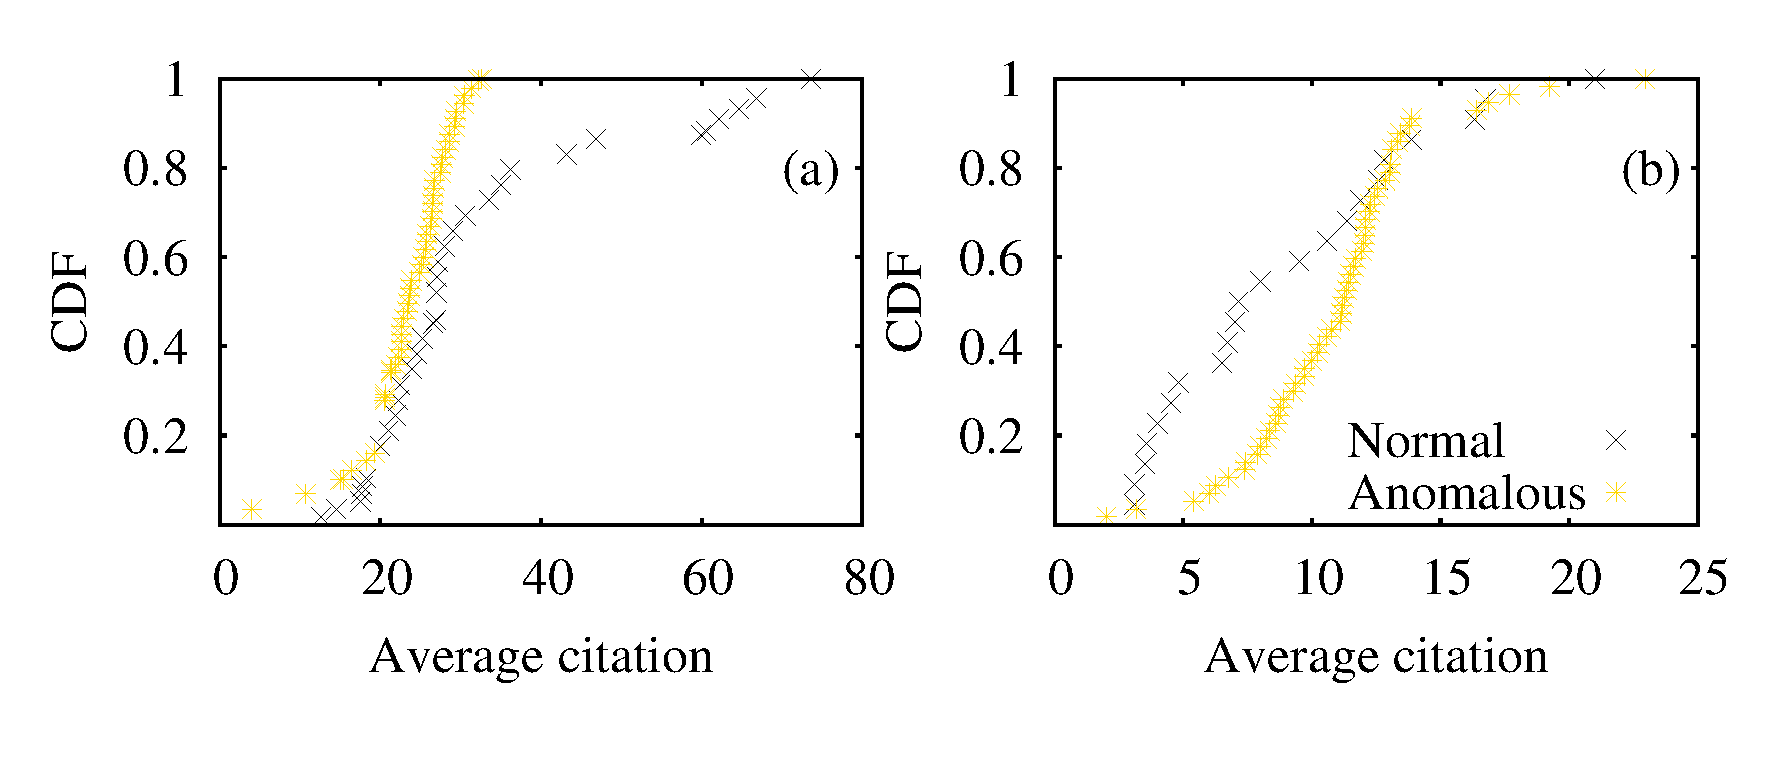
\includegraphics[scale=0.27]{./texfiles/Chapter_4/cikm/figures/editor_all_anom.eps}
\caption{\label{ed_pred}Cumulative distribution function of the average citations for the two sets of editors (anomalous and normal).} 
%\vspace{-.4cm}
\end{figure}


\subsection{Editors}
For each editor $i$, we measure $MEAT_{i}$, $RDI_{i}$, $RADI_{i}$ and $SRI_{i}$ which form a feature vector. 
%[{\color{red}{\bf Have you not used $SRI$? Why?}}] 
We also consider the editors who were assigned at least 5 papers and accepted at least 1 paper before 2013. 
To detect anomalies we use the 
$k-means$ clustering setting with $k=2$. The two clusters are of sizes 25 and 68 respectively. Clearly this set of 25 editors are the anomalous ones.
In figure \ref{ed_pred} we plot the cumulative distribution of average citation of accepted (figure \ref{ed_pred}(a)) and rejected  (figure \ref{ed_pred}(b)) papers. We observe that citation of accepted papers assigned to anomalous editors are significantly lower while citation of rejected papers are significantly higher compared to those assigned to normal editors.


\subsection{Reviewers}

Similarly for each reviewer $i$ we associate a feature vector of size seven consisting of $MRAT_{i}$, $MRSD_{i}$, $TDI_{i}$, $EDI_{i}$, $AR_{i}$, $MTD_{i}$ and $DFI_{i}$. 
%[{\color{red}{\bf Have you not used $DFI$? Why?}}] 
We filter out reviewers who have reviewed at least 5 papers and accepted at least 1 before 2013. This reduces our set of reviewers to 2328. By using $k-means$ clustering ($k=2$), we obtain two clusters of size 339 and 
1999. On plotting cumulative distribution of the average citation for accepted (refer to figure \ref{rev_pred}(a)) and rejected papers (refer to figure \ref{rev_pred}(b)), we observe that the papers accepted by anomalous reviewers are cited significantly lesser while those rejected by them are cited significantly higher compared to the normal referees.

\begin{figure}
\centering
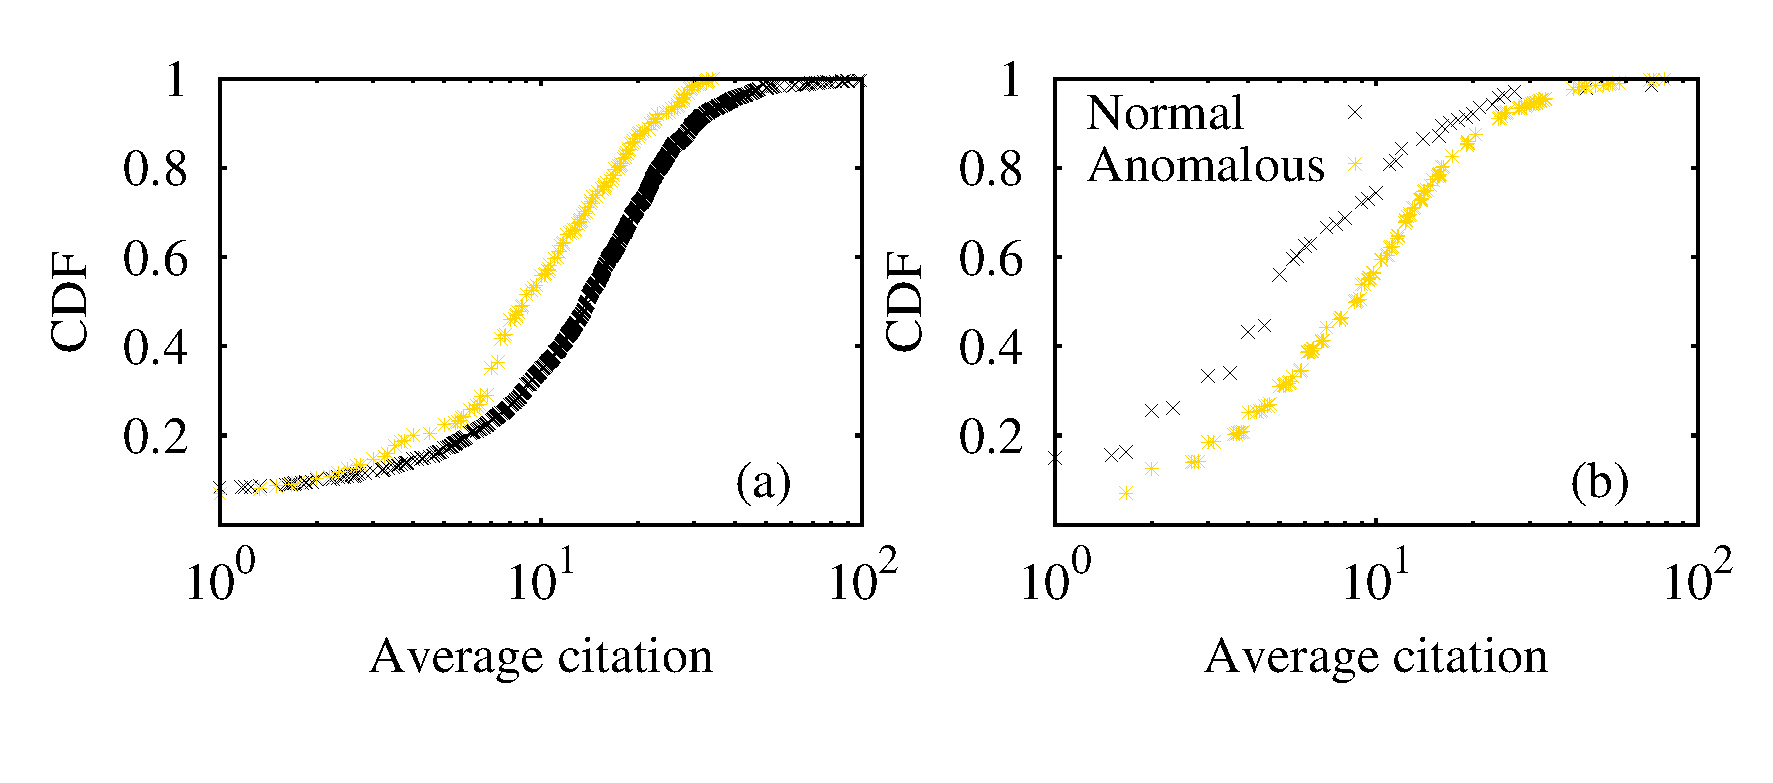
\includegraphics[scale=0.4]{./texfiles/Chapter_4/cikm/figures/reviewer_all_anom.eps}
\caption{\label{rev_pred}Cumulative distribution function of the average citations for the two sets of reviewers (anomalous and normal).}
%\vspace{-.4cm}
\end{figure}


%\begin{figure}
\centering
\includegraphics[scale=0.25]{./texfiles/Chapter_4/jcdl/figures/len_citation.eps}
\caption{Mean length of referee reports in terms of number of words at different rounds of review. Typically the buckets are $< 100$, ($\geq 100, < 200$) and so on}
\label{fig:length}
\end{figure}


\subsection{Review report based features}
\label{text_analysis}

In this subsection we analyze whether certain features could be extracted from the reports sent by the reviewers that could be an indicator of the long-term citation of the paper. Note that we have two types of reports -- {\bf Referee report}: Report sent by the assigned referee to the editors and {\bf Editor report}: Report sent by the editor to the authors based on the referee report. We primarily focus on the referee reports as editorial reports are in almost all cases a reiteration of the referee reports.

\subsubsection{Length of the reports (RL)}
We start by looking whether the length of the review reports sent by the reviewers are indicative of the quality and hence the long-term citation of the paper. To this aim we segregate the papers based on the length of the report and calculate the mean citation of each of these buckets. The lengths are bucketed with sizes typically $< 100$, ($\geq 100, < 200$) and so on. We observe that there exists an optimal length (between 500 and 600 words) for which the citation obtained by the corresponding paper is maximum  (refer to figure \ref{fig:length}). 


\subsubsection{Sentiments (SNT)}
We next perform sentiment analysis on the review reports. To determine the sentiment of a report we use a method described in~\cite{montejo2012random} which performs a graph-based word sense disambiguation and lexical similarity analysis using a pre-existing knowledge base. A sentiment score of 0 indicates that the document is neutral, a positive score  indicates a positive sentiment and a negative score indicates a negative sentiment. 


\begin{figure}[htpb]
\centering
%\vspace{-5mm}
\includegraphics[scale=0.23]{./texfiles/Chapter_4/jcdl/figures/year_sent_cit-eps-converted-to.pdf}
\caption{Sentiment score versus citations for both accepted and rejected papers for the years 2005, 2007 and 2009. We find similar trends for other years as well.}
\label{fig12}
\end{figure}

To determine whether the overall sentiment of the reviews of a paper is related to the number of citations received by it, we plot for each paper (both accepted and rejected) the number of citations it received against the  sentiment score of the first round of review in fig.~\ref{fig12}. Note that we segregate the papers based on the year of the publication or the rejection. We observe that the highly cited papers mostly have reviews with neutral or positive sentiment. Accepted papers with positive reviews are, on average, found to receive $25.27$ citations while those with negative reviews are found to receive $13.56$ citations.
However, there are cases where the accepted paper received highly positive reviews but was not cited. Conversely, there are cases where the sentiment was neutral but the paper garnered a large number of citations. Shown below are two such examples -- {\bf Case 1:} Year of publication: 2006, sentiment score: 0.0234 (almost neutral), citations: 5812; {\bf Case 2:} Year of publication: 2008, sentiment score: 0.65 (highly positive), citations: 6.


For the rejected papers we observe that those which received neutral reviews but were rejected, tend to garner higher citations later compared to the ones which received negative reviews. There are certain exceptions as well, two of which are -- {\bf Case 1:} Year of rejection: 2010, sentiment score: 0.27 (positive), citations: 1; {\bf Case 2:} Year of rejection: 2007, sentiment score: -0.14 (negative), citations: 711.
Manual investigation of the review text shows that the papers which are highly cited after rejection were mainly rejected for not being in the scope of JHEP and not because of flawed results. 

\subsubsection{Linguistic quality indicators (LQI)}

Here we check whether there are linguistic quality features present in the review reports which can serve as an indicator of the future impact of the paper. To our aim we use the LIWC\footnote{\url{http://liwc.wpengine.com/}} (Linguistic Inquiry and Word Count) text analysis tool~\cite{pennebaker2007development}. The tool provides, as output, percentage of words in different categories for an input text. The categories are broadly divided into linguistic (21 dimensions like pronouns, articles etc.), psychological (41 dimensions like affect, cognition etc.), personal concern (6 dimensions), informal language markers and punctuation apart from some general features like word count, words per sentence etc. We apply the LIWC tool on the review reports for our analysis and mainly focus on the linguistic and the psychological categories.
Next we check whether the LIWC features discussed earlier can also serve as indicators differentiating high and low cited papers. We rank the papers based on the number of citations they have received and consider the top 10\% as highly cited and the bottom 10\% as low cited papers. Note that we only consider the papers that were published before 2012 so that the papers have at least three years of citation history. In table~\ref{tab3} we report the mean percentage of words in different LIWC categories across all the papers (both high and low cited). We find several quality indicators here as well. The key observations are: (i) future tense is used more significantly in case of review reports of highly cited papers compared to low cited papers. On manually investigating the reviews of some of the highly cited papers we observe that statements like ``its result will become a useful addition to ..'' are prevalent; (ii) insightful and inclusive words are also used to a greater extent in review reports of highly cited papers compared to low cited papers; (iii) positive words are also more prevalent in highly cited papers as well.\\
Thus, these indicators show that the reviewers were, in many cases, indeed able to guess the quality of the paper as is evident from the review reports.

\begin{table}
\centering
\caption{Mean values of percentages of various categories of words in review reports of high and low cited papers where the means differ significantly.\vspace{3mm}}
\label{tab3}
\begin{tabular}{|l|l|l|l|}
\hline
Category                    & Dimension                                                   & \begin{tabular}[c]{@{}l@{}}High cited\\ papers\end{tabular} & \begin{tabular}[c]{@{}l@{}}Low cited\\ papers\end{tabular} \\ \hline \hline
\multirow{2}{*}{Linguistic} & Future tense                                                & 1.17                                                          & 1.05                                                         \\ \cline{2-4} 
                            & Negation                                                    & 0.72                                                          & 0.84                                                         \\ \hline
\multirow{4}{*}{Cognitive}  & Insight                                                     & 3.52                                                          & 3.16                                                         \\ \cline{2-4} 
                            & Causation                                                   & 2.60                                                          & 2.38                                                         \\ \cline{2-4} 
                            & Inclusive                                                   & 3.70                                                          & 3.43                                                         \\ \cline{2-4} 
                            & Exclusive                                                   & 1.28                                                          & 1.52                                                         \\ \hline
Affective                   & \begin{tabular}[c]{@{}l@{}}Positive \\ emotion\end{tabular} & 2.84                                                          & 2.70                                                         \\ \hline
\end{tabular}
\vspace{2mm}
\end{table}


%\noindent
\section{Profiling Anomalous Reviewers}
\label{profile}


In this section we analyze in more details the performance of the anomalous reviewers. To this aim, we consider for each reviewer, the sequence of papers accepted by her and the citation accrued (within the first three years from publication) by each of these papers. A decreasing trend would suggest decline in performance of the reviewer. Depending on the trend we observe three broad categories within the set of anomalous reviewers \\
(i) performance deteriorates constantly over time (proportion = $42.5\%$, figure \ref{cit_prof}(a)).\\
(ii) performance is good for initial few papers but deteriorates in the long run (proportion = $22.6\%$, figure \ref{cit_prof}(b)).\\
(iii) performance fluctuates but has a deteriorating trend in the long run (proportion = $34.9\%$, figure \ref{cit_prof}(c)).
\begin{figure}
\centering
\includegraphics[scale=0.3]{./texfiles/Chapter_4/cikm/figures/profile_all.eps}
\caption{\label{cit_prof} Mean citation profile of the reviewers in the three categories.}
\end{figure}

%Thus, for almost all the reviewers in the anomalous category, we observe that the performance degrades over time which further supports the observation that the anomalous reviewers usually tend to under-perform over time.
\medskip

\section{Profiling Anomalous Reviewers}
\label{profile}


In this section we analyze in more details the performance of the anomalous reviewers. To this aim, we consider for each reviewer, the sequence of papers accepted by her and the citation accrued (within the first three years from publication) by each of these papers. A decreasing trend would suggest decline in performance of the reviewer. Depending on the trend we observe three broad categories within the set of anomalous reviewers \\
(i) performance deteriorates constantly over time (proportion = $42.5\%$, figure \ref{cit_prof}(a)).\\
(ii) performance is good for initial few papers but deteriorates in the long run (proportion = $22.6\%$, figure \ref{cit_prof}(b)).\\
(iii) performance fluctuates but has a deteriorating trend in the long run (proportion = $34.9\%$, figure \ref{cit_prof}(c)).
\begin{figure}
\centering
\includegraphics[scale=0.4]{./texfiles/Chapter_4/cikm/figures/profile_all.eps}
\caption{\label{cit_prof} Mean citation profile of the reviewers in the three categories.}
%\vspace{-.4cm}
\end{figure}

%\noindent
We in this paper performed a detailed comparative analysis of cases where a single reviewer was involved in the peer-review process and where multiple reviewers were involved, considering the review history of papers submitted to two leading journals of physics (JHEP and JSTAT). 
%Although multiple reviewers are generally preferred over a single reviewer, 
We made an interesting observation  that accepted papers which were reviewed by a single referee on average tend to garner a larger number of citations in 
long term compared to those which were reviewed by multiple referees. An exact opposite behavior is observed in case of rejected papers. 

Through a more detailed analysis, we however observed several contradictory trends - although on average single reviewers perform better, however, 
most impactful papers are largely multi-refereed;  the multi-refereed papers generally perform poorly due to discordance between the reviewers.
Further we tried to understand the reason behind under-performance and found that frequent assigning of review to a reviewer leads to his performance deterioration. 
Also those reviewers who have a tendency to be too critical or too liberal fail to identify the real good papers. 

A real problem in the process of reviewing is the scarcity of reviewers, hence discarding under-performing reviewers may not be a practical solution. 
So we checked the performance of these reviewers with high-graded reviewers and find that the quality is much better than their normal average. Hence a 
technique would be to combine high and low graded reviewers intelligently. 

\if{0}
 of review reports of referees in a multi-review cases we observed that the referees often contradict each other. On analyzing the behavior of the editors and the referees, we further observed that - \\
(i) Anomalous editors on average tend to assign multiple reviewers compared to the normal ones. Furthermore they tend to assign at least one anomalous reviewer among the multiple reviewers. \\
(ii) Anomalous reviewers when part of a multi-reviewer set up tend to perform better compared to being assigned as a single reviewer.\\

We further proposed to quantify the fitness of the referees based on the time till his last assignment and his accept ratio. 
\fi
Based on the observations above, we proposed a scheme based on genetic algorithm to recommend reviewer groups to the editors 
to make reviewer assignments. In fact our system was correctly able to recommend reviewer groups in $\sim$ 78\% cases across the two datasets.
%$78.25\%$ of cases for JHEP and $76.5\%$ of cases for JSTAT.

\if{0}
We further showed that the importance of editor's intervention to the effectiveness of our  proposed framework in long term. 
\subsubsection{Future directions}
Our current work points out to several future directions which we plan to explore in subsequent works. In its current state our algorithm only recommends referees from an already existing set. An immediate extension is to identify mechanisms to handle new referees in the system. In future, we would also like to test our recommendation system in a real settings and observe if indeed the performance of peer-review is enhanced. We believe our findings would make the scientific peer-review system much more effective.
\fi

\medskip


\section{Conclusion}
\label{conclusion}

In this paper we provided a framework for identifying anomalous reviewers and editors based on  their review history considering Journal of High Energy Physics as a case study. We identified several factors that are indicative of anomalous behavior of the editors as well as reviewers. In specific for editors we observed that - 
(i) high frequency of assignment, (ii) selecting from a very small set of referees for reviewing, (iii) assigning same reviewer to papers of same author and (iv) assigning herself as reviewer instead of assigning someone else could be indicative of anomalous behavior of the editor. 

Similarly for reviewers we observe that - 
(i) high frequency of assignment, (ii) delay in sending report, (iii) assignment from only a single editor or a very small set of editors (iv) 
very high or very low acceptance ratio and (vi) delay in notifying the editor about her decision to decline are also indicative of anomalous behavior and often leads to under-performance. Based on these factors we were able to identify anomalous referees and editors using an unsupervised clustering approach. 

\noindent{\bf Future directions:} We believe our findings could be useful in better assignment of editors and reviewers and thereby improve the performance of the peer-review system. Assigning good reviewers is an important part of the peer-review process and our findings allow for identifying under-performing referees. This could be a first step towards developing a reviewer-recommendation system whereby the editors are recommended a set of reviewers based on their performance. 
We plan to come up with such a system in subsequent works.

%
\noindent
I would like to take this opportunity express my gratitude to everybody who have inspired me and contributed directly or indirectly in realizing this
thesis. My parents have been the greatest source of inspiration and strength throughout my life and without their support and sacrifice, this thesis would never have taken shape. I would also like to thank my elder brother who has been my mentor throughout my life.     

It is impossible to express my gratitude to my supervisors, Prof.
Animesh Mukherjee and Prof. Niloy Ganguly in a few words. The long discussions with them not only helped me in formulating the problems of this thesis, but
also helped me to understand the nuances of doing research. This thesis would never have been possible without their constant support and encouragement. 
I would like to thank Dr. Matteo Marsili (ICTP, Italy) and Dr. Tyll Krueger (Wroclaw University of Science and Technology) for their guidance and support. 
I would also like to thank the members of my DSC Prof. J. Mukhopadhyay, Prof. A. Basu, Prof. D. Mukhopadhyay and Prof. A. Mukherjee  who have enriched this thesis with their insights and suggestions. 

I consider myself very fortunate to have been part of Complex Network Research Group (CNeRG). At CNeRG I have had the pleasure of knowing Parantapa Bhattacharya, Abir Dey, Surjya Ghosh, Tanmoy Chakraborty, Suman Kalyan Maity, Soumajit Pramanik, Abhik Jana, Sankarshan Mridha, Abhijnan Chakraborty, Ankan Mullick, Satadal Sengupta, Rohit Verma, Madhumita Mallick, Rijula Kar, Amrit Krishna, Mayank Singh, Subhendu Khatuya, Soumya Sarkar and Kaustav Rudra. Life would not have been same without them. I should also thank Debojyoti Kundu who has been a great roommate and a close friend.     

Lastly, this long journey has not always been smooth but has revealed to me the joy of learning and my only desire is to pursue it for the rest of my life. 

%realize that it is not success or fame but the sheer joy of learning that drives me to work every morning and my only desire is to continue it for the rest of my life.  








\if{0}
\section*{Acknowledgment}
We would like to thank publication team of Journal of High Energy Physics (JHEP) for providing us the necessary data and they were the only ones willing to provide it.

%\bibliographystyle{abbrv}
%\bibliography{sigproc}

\begin{thebibliography}{10}

\bibitem{bacchetti2002peer}
P.~Bacchetti.
\newblock Peer review of statistics in medical research: the other problem.
\newblock {\em British Medical Journal}, 324(7348):1271, 2002.

\bibitem{braatz2014papers}
R.~D. Braatz.
\newblock Papers receive more citations after rejection [publication
  activities].
\newblock {\em Control Systems, IEEE}, 34(4):22--23, 2014.

\bibitem{caswellimproving}
H.~Caswell.
\newblock Improving peer review.

\bibitem{chandola2009anomaly}
V.~Chandola, A.~Banerjee, and V.~Kumar.
\newblock Anomaly detection: A survey.
\newblock {\em ACM computing surveys (CSUR)}, 41(3):15, 2009.

\bibitem{cole1981chance}
S.~Cole, G.~A. Simon, et~al.
\newblock Chance and consensus in peer review.
\newblock {\em Science}, 214(4523):881--886, 1981.

\bibitem{garfield1999journal}
E.~Garfield.
\newblock Journal impact factor: a brief review.
\newblock {\em Canadian Medical Association Journal}, 161(8):979--980, 1999.

\bibitem{graffy2006improving}
J.~Graffy, R.~Bryar, S.~Kendall, and D.~Crook.
\newblock Improving peer review.
\newblock {\em Primary Health Care Research and Development}, 7(01):1--2, 2006.

\bibitem{hartigan1979algorithm}
J.~A. Hartigan and M.~A. Wong.
\newblock Algorithm as 136: A k-means clustering algorithm.
\newblock {\em Journal of the Royal Statistical Society. Series C (Applied
  Statistics)}, 28(1):100--108, 1979.

\bibitem{ingelfinger1974peer}
F.~J. Ingelfinger.
\newblock Peer review in biomedical publication.
\newblock {\em The American journal of medicine}, 56(5):686--692, 1974.

\bibitem{kassirer1994peer}
J.~P. Kassirer and E.~W. Campion.
\newblock Peer review: crude and understudied, but indispensable.
\newblock {\em JAMA}, 272(2):96--97, 1994.

\bibitem{mcnutt1990effects}
R.~A. McNutt, A.~T. Evans, R.~H. Fletcher, and S.~W. Fletcher.
\newblock The effects of blinding on the quality of peer review: a randomized
  trial.
\newblock {\em JAMA}, 263(10):1371--1376, 1990.

\bibitem{relman1989good}
A.~S. Relman and M.~Angell.
\newblock How good is peer review?
\newblock {\em The New England journal of medicine}, 321(12):827--829, 1989.

\bibitem{smith2006peer}
R.~Smith.
\newblock Peer review: a flawed process at the heart of science and journals.
\newblock {\em Journal of the royal society of medicine}, 99(4):178--182, 2006.

\end{thebibliography}

\end{document}
\fi